\documentclass[twoside]{book}

% Packages required by doxygen
\usepackage{fixltx2e}
\usepackage{calc}
\usepackage{doxygen}
\usepackage[export]{adjustbox} % also loads graphicx
\usepackage{graphicx}
\usepackage[utf8]{inputenc}
\usepackage{makeidx}
\usepackage{multicol}
\usepackage{multirow}
\PassOptionsToPackage{warn}{textcomp}
\usepackage{textcomp}
\usepackage[nointegrals]{wasysym}
\usepackage[table]{xcolor}

% Font selection
\usepackage[T1]{fontenc}
\usepackage[scaled=.90]{helvet}
\usepackage{courier}
\usepackage{amssymb}
\usepackage{sectsty}
\renewcommand{\familydefault}{\sfdefault}
\allsectionsfont{%
  \fontseries{bc}\selectfont%
  \color{darkgray}%
}
\renewcommand{\DoxyLabelFont}{%
  \fontseries{bc}\selectfont%
  \color{darkgray}%
}
\newcommand{\+}{\discretionary{\mbox{\scriptsize$\hookleftarrow$}}{}{}}

% Page & text layout
\usepackage{geometry}
\geometry{%
  a4paper,%
  top=2.5cm,%
  bottom=2.5cm,%
  left=2.5cm,%
  right=2.5cm%
}
\tolerance=750
\hfuzz=15pt
\hbadness=750
\setlength{\emergencystretch}{15pt}
\setlength{\parindent}{0cm}
\setlength{\parskip}{3ex plus 2ex minus 2ex}
\makeatletter
\renewcommand{\paragraph}{%
  \@startsection{paragraph}{4}{0ex}{-1.0ex}{1.0ex}{%
    \normalfont\normalsize\bfseries\SS@parafont%
  }%
}
\renewcommand{\subparagraph}{%
  \@startsection{subparagraph}{5}{0ex}{-1.0ex}{1.0ex}{%
    \normalfont\normalsize\bfseries\SS@subparafont%
  }%
}
\makeatother

% Headers & footers
\usepackage{fancyhdr}
\pagestyle{fancyplain}
\fancyhead[LE]{\fancyplain{}{\bfseries\thepage}}
\fancyhead[CE]{\fancyplain{}{}}
\fancyhead[RE]{\fancyplain{}{\bfseries\leftmark}}
\fancyhead[LO]{\fancyplain{}{\bfseries\rightmark}}
\fancyhead[CO]{\fancyplain{}{}}
\fancyhead[RO]{\fancyplain{}{\bfseries\thepage}}
\fancyfoot[LE]{\fancyplain{}{}}
\fancyfoot[CE]{\fancyplain{}{}}
\fancyfoot[RE]{\fancyplain{}{\bfseries\scriptsize Generated by Doxygen }}
\fancyfoot[LO]{\fancyplain{}{\bfseries\scriptsize Generated by Doxygen }}
\fancyfoot[CO]{\fancyplain{}{}}
\fancyfoot[RO]{\fancyplain{}{}}
\renewcommand{\footrulewidth}{0.4pt}
\renewcommand{\chaptermark}[1]{%
  \markboth{#1}{}%
}
\renewcommand{\sectionmark}[1]{%
  \markright{\thesection\ #1}%
}

% Indices & bibliography
\usepackage{natbib}
\usepackage[titles]{tocloft}
\setcounter{tocdepth}{3}
\setcounter{secnumdepth}{5}
\makeindex

% Hyperlinks (required, but should be loaded last)
\usepackage{ifpdf}
\ifpdf
  \usepackage[pdftex,pagebackref=true]{hyperref}
\else
  \usepackage[ps2pdf,pagebackref=true]{hyperref}
\fi
\hypersetup{%
  colorlinks=true,%
  linkcolor=blue,%
  citecolor=blue,%
  unicode%
}

% Custom commands
\newcommand{\clearemptydoublepage}{%
  \newpage{\pagestyle{empty}\cleardoublepage}%
}

\usepackage{caption}
\captionsetup{labelsep=space,justification=centering,font={bf},singlelinecheck=off,skip=4pt,position=top}

%===== C O N T E N T S =====

\begin{document}

% Titlepage & ToC
\hypersetup{pageanchor=false,
             bookmarksnumbered=true,
             pdfencoding=unicode
            }
\pagenumbering{alph}
\begin{titlepage}
\vspace*{7cm}
\begin{center}%
{\Large Train-\/\+System }\\
\vspace*{1cm}
{\large Generated by Doxygen 1.8.14}\\
\end{center}
\end{titlepage}
\clearemptydoublepage
\pagenumbering{roman}
\tableofcontents
\clearemptydoublepage
\pagenumbering{arabic}
\hypersetup{pageanchor=true}

%--- Begin generated contents ---
\chapter{Hierarchical Index}
\section{Class Hierarchy}
This inheritance list is sorted roughly, but not completely, alphabetically\+:\begin{DoxyCompactList}
\item \contentsline{section}{Date}{\pageref{classDate}}{}
\item \contentsline{section}{Engineer\+:\+:Engineer\+Hash\+Utils}{\pageref{structEngineer_1_1EngineerHashUtils}}{}
\item exception\begin{DoxyCompactList}
\item \contentsline{section}{Identical\+Destination\+Exception}{\pageref{classIdenticalDestinationException}}{}
\item \contentsline{section}{Invalid\+Date\+Exception}{\pageref{classInvalidDateException}}{}
\item \contentsline{section}{Invalid\+Train\+Type\+Exception}{\pageref{classInvalidTrainTypeException}}{}
\item \contentsline{section}{No\+Such\+Engineer\+Exception}{\pageref{classNoSuchEngineerException}}{}
\item \contentsline{section}{No\+Such\+Passenger\+Exception}{\pageref{classNoSuchPassengerException}}{}
\item \contentsline{section}{No\+Such\+Station\+Exception}{\pageref{classNoSuchStationException}}{}
\item \contentsline{section}{No\+Such\+Train\+Exception}{\pageref{classNoSuchTrainException}}{}
\item \contentsline{section}{No\+Such\+Trip\+Exception}{\pageref{classNoSuchTripException}}{}
\item \contentsline{section}{Reverse\+Dates\+Exception}{\pageref{classReverseDatesException}}{}
\item \contentsline{section}{Trip\+Past\+Exception}{\pageref{classTripPastException}}{}
\end{DoxyCompactList}
\item \contentsline{section}{Passenger\+Card}{\pageref{classPassengerCard}}{}
\item \contentsline{section}{Purchase\+Log}{\pageref{classPurchaseLog}}{}
\item \contentsline{section}{Repair\+Shop\+:\+:Repair\+Shop\+P\+Q\+Utils}{\pageref{structRepairShop_1_1RepairShopPQUtils}}{}
\item \contentsline{section}{System}{\pageref{classSystem}}{}
\item \contentsline{section}{System\+Element}{\pageref{classSystemElement}}{}
\begin{DoxyCompactList}
\item \contentsline{section}{Person}{\pageref{classPerson}}{}
\begin{DoxyCompactList}
\item \contentsline{section}{Engineer}{\pageref{classEngineer}}{}
\item \contentsline{section}{Passenger}{\pageref{classPassenger}}{}
\end{DoxyCompactList}
\item \contentsline{section}{Repair\+Shop}{\pageref{classRepairShop}}{}
\item \contentsline{section}{Station}{\pageref{classStation}}{}
\item \contentsline{section}{Train}{\pageref{classTrain}}{}
\begin{DoxyCompactList}
\item \contentsline{section}{Alfa\+Pendular}{\pageref{classAlfaPendular}}{}
\item \contentsline{section}{Inter\+Cidades}{\pageref{classInterCidades}}{}
\end{DoxyCompactList}
\item \contentsline{section}{Trip}{\pageref{classTrip}}{}
\end{DoxyCompactList}
\item \contentsline{section}{Ticket\+Invoice}{\pageref{classTicketInvoice}}{}
\item \contentsline{section}{Ticket\+Purchase\+Request}{\pageref{classTicketPurchaseRequest}}{}
\end{DoxyCompactList}

\chapter{Class Index}
\section{Class List}
Here are the classes, structs, unions and interfaces with brief descriptions\+:\begin{DoxyCompactList}
\item\contentsline{section}{\mbox{\hyperlink{classDate}{Date}} \\*Class for representing dates in the program }{\pageref{classDate}}{}
\item\contentsline{section}{\mbox{\hyperlink{classPassenger}{Passenger}} \\*Class for representing a passenger in the system }{\pageref{classPassenger}}{}
\item\contentsline{section}{\mbox{\hyperlink{classPassengerCard}{Passenger\+Card}} \\*Class for representing the card of a passenger in the system }{\pageref{classPassengerCard}}{}
\item\contentsline{section}{\mbox{\hyperlink{classPurchaseLog}{Purchase\+Log}} }{\pageref{classPurchaseLog}}{}
\item\contentsline{section}{\mbox{\hyperlink{classStation}{Station}} \\*Class for representing a station in the system }{\pageref{classStation}}{}
\item\contentsline{section}{\mbox{\hyperlink{classSystem}{System}} \\*Class to represent the central system }{\pageref{classSystem}}{}
\item\contentsline{section}{\mbox{\hyperlink{classTicketInvoice}{Ticket\+Invoice}} \\*Class for representing an invoice of a ticket purchase in the system }{\pageref{classTicketInvoice}}{}
\item\contentsline{section}{\mbox{\hyperlink{classTicketPurchaseRequest}{Ticket\+Purchase\+Request}} \\*Class to represent a ticket purchase request }{\pageref{classTicketPurchaseRequest}}{}
\item\contentsline{section}{\mbox{\hyperlink{classTrain}{Train}} \\*Class for representing a train in the system }{\pageref{classTrain}}{}
\item\contentsline{section}{\mbox{\hyperlink{classTrip}{Trip}} \\*Class for representing a trip in the system }{\pageref{classTrip}}{}
\end{DoxyCompactList}

\chapter{Class Documentation}
\hypertarget{classDate}{}\section{Date Class Reference}
\label{classDate}\index{Date@{Date}}


Class for representing dates in the program.  




{\ttfamily \#include $<$Date.\+h$>$}

\subsection*{Public Member Functions}
\begin{DoxyCompactItemize}
\item 
\mbox{\hyperlink{classDate_aa29ee0f04162437b91b758be0a4b75fc}{Date}} (int year, int month, int day, int hour=0, int minute=0)
\begin{DoxyCompactList}\small\item\em Construct a new \mbox{\hyperlink{classDate}{Date}} object. \end{DoxyCompactList}\item 
\mbox{\hyperlink{classDate_abaa8b0cf93eb1ad9206be4ff78ed2a3b}{Date}} (const std\+::string \&date\+String)
\begin{DoxyCompactList}\small\item\em Construct a new \mbox{\hyperlink{classDate}{Date}} object. \end{DoxyCompactList}\item 
bool \mbox{\hyperlink{classDate_a91ccc0361527f5f68785c5460d750a12}{operator==}} (\mbox{\hyperlink{classDate}{Date}} \&d)
\begin{DoxyCompactList}\small\item\em Check eqaulity between \mbox{\hyperlink{classDate}{Date}} objects. \end{DoxyCompactList}\item 
bool \mbox{\hyperlink{classDate_a51d1dadde23783adc9a2ae12d877803c}{operator$<$}} (\mbox{\hyperlink{classDate}{Date}} \&d)
\begin{DoxyCompactList}\small\item\em Check if \mbox{\hyperlink{classDate}{Date}} object happens before argument. \end{DoxyCompactList}\item 
bool \mbox{\hyperlink{classDate_a49b4e0ed6752c928164fd483720423da}{operator$<$=}} (\mbox{\hyperlink{classDate}{Date}} \&d)
\begin{DoxyCompactList}\small\item\em Check if \mbox{\hyperlink{classDate}{Date}} object happens before or at same time as argument. \end{DoxyCompactList}\item 
bool \mbox{\hyperlink{classDate_a0c2a1a6f890da1f9a360fab87e7109a3}{operator$>$}} (\mbox{\hyperlink{classDate}{Date}} \&d)
\begin{DoxyCompactList}\small\item\em Check if \mbox{\hyperlink{classDate}{Date}} object happens after argument. \end{DoxyCompactList}\item 
bool \mbox{\hyperlink{classDate_a3dd4c3c4818d69669927bec072ff85ce}{operator$>$=}} (\mbox{\hyperlink{classDate}{Date}} \&d)
\begin{DoxyCompactList}\small\item\em Check if \mbox{\hyperlink{classDate}{Date}} object happens after or at same time as argument. \end{DoxyCompactList}\item 
std\+::string \mbox{\hyperlink{classDate_a733c89177097f0d7f5cc2f68f5593856}{get\+Date\+String}} () const
\begin{DoxyCompactList}\small\item\em Get the \mbox{\hyperlink{classDate}{Date}} String. \end{DoxyCompactList}\item 
std\+::string \mbox{\hyperlink{classDate_a54b53336c8ba897fae4d2bbb0aa84a99}{get\+Date\+String\+Without\+Hours}} () const
\begin{DoxyCompactList}\small\item\em Get the \mbox{\hyperlink{classDate}{Date}} String Without Hours. \end{DoxyCompactList}\item 
int \mbox{\hyperlink{classDate_a8b0869f34c2b38d108ab83ee2e770e5d}{get\+Year}} () const
\begin{DoxyCompactList}\small\item\em Get the Year. \end{DoxyCompactList}\item 
int \mbox{\hyperlink{classDate_a332f6e3a2f6a40d73742b6dab7be0f64}{get\+Month}} () const
\begin{DoxyCompactList}\small\item\em Get the Month. \end{DoxyCompactList}\item 
int \mbox{\hyperlink{classDate_a0f253815240e70f4c39cb93cc68bd3f4}{get\+Day}} () const
\begin{DoxyCompactList}\small\item\em Get the Day. \end{DoxyCompactList}\item 
int \mbox{\hyperlink{classDate_ab8ea9e1aafa6cb95be7b82cda0c53cfe}{get\+Hour}} () const
\begin{DoxyCompactList}\small\item\em Get the Hour. \end{DoxyCompactList}\item 
int \mbox{\hyperlink{classDate_a55251df891f43b9f19419cd79ce69876}{get\+Minutes}} () const
\begin{DoxyCompactList}\small\item\em Get the Minutes. \end{DoxyCompactList}\item 
long int \mbox{\hyperlink{classDate_af047ef9ca2cf7843b921f36e9883f0a7}{get\+Time\+Stamp}} ()
\begin{DoxyCompactList}\small\item\em Get the Time Stamp object. \end{DoxyCompactList}\end{DoxyCompactItemize}
\subsection*{Friends}
\begin{DoxyCompactItemize}
\item 
std\+::ostream \& \mbox{\hyperlink{classDate_a2f114c7aa1398dac0f21b888bcb40f3e}{operator$<$$<$}} (std\+::ostream \&o, \mbox{\hyperlink{classDate}{Date}} \&d)
\begin{DoxyCompactList}\small\item\em ouput \mbox{\hyperlink{classDate}{Date}} object into an output stream \end{DoxyCompactList}\end{DoxyCompactItemize}


\subsection{Detailed Description}
Class for representing dates in the program. 

Works as an abstraction of C++\textquotesingle{}s ctime library. 

\subsection{Constructor \& Destructor Documentation}
\mbox{\Hypertarget{classDate_aa29ee0f04162437b91b758be0a4b75fc}\label{classDate_aa29ee0f04162437b91b758be0a4b75fc}} 
\index{Date@{Date}!Date@{Date}}
\index{Date@{Date}!Date@{Date}}
\subsubsection{\texorpdfstring{Date()}{Date()}\hspace{0.1cm}{\footnotesize\ttfamily [1/2]}}
{\footnotesize\ttfamily Date\+::\+Date (\begin{DoxyParamCaption}\item[{int}]{year,  }\item[{int}]{month,  }\item[{int}]{day,  }\item[{int}]{hour = {\ttfamily 0},  }\item[{int}]{minute = {\ttfamily 0} }\end{DoxyParamCaption})}



Construct a new \mbox{\hyperlink{classDate}{Date}} object. 

Constructs \mbox{\hyperlink{classDate}{Date}} object and calls validate(). If validation fails, throws Invalid\+Date\+Exception.


\begin{DoxyParams}{Parameters}
{\em year} & \mbox{\hyperlink{classDate}{Date}}\textquotesingle{}s year \\
\hline
{\em month} & \mbox{\hyperlink{classDate}{Date}}\textquotesingle{}s month \\
\hline
{\em day} & \mbox{\hyperlink{classDate}{Date}}\textquotesingle{}s day in month \\
\hline
{\em hour} & \mbox{\hyperlink{classDate}{Date}}\textquotesingle{}s hour of day (24h format) \\
\hline
{\em minute} & \mbox{\hyperlink{classDate}{Date}}\textquotesingle{}s minutes \\
\hline
\end{DoxyParams}
\mbox{\Hypertarget{classDate_abaa8b0cf93eb1ad9206be4ff78ed2a3b}\label{classDate_abaa8b0cf93eb1ad9206be4ff78ed2a3b}} 
\index{Date@{Date}!Date@{Date}}
\index{Date@{Date}!Date@{Date}}
\subsubsection{\texorpdfstring{Date()}{Date()}\hspace{0.1cm}{\footnotesize\ttfamily [2/2]}}
{\footnotesize\ttfamily Date\+::\+Date (\begin{DoxyParamCaption}\item[{const std\+::string \&}]{date\+String }\end{DoxyParamCaption})}



Construct a new \mbox{\hyperlink{classDate}{Date}} object. 

Constructs \mbox{\hyperlink{classDate}{Date}} object and calls validate(). If validation fails, throws Invalid\+Date\+Exception.


\begin{DoxyParams}{Parameters}
{\em date\+String} & \mbox{\hyperlink{classDate}{Date}} in form of a string in format \char`\"{}dd-\/mm-\/yyyy H\+H\+:\+M\+M\char`\"{}. Day, month, year, hour and minutes must be two digits (\textquotesingle{}02\textquotesingle{}, \textquotesingle{}08\textquotesingle{}, \textquotesingle{}12\textquotesingle{}) \\
\hline
\end{DoxyParams}


\subsection{Member Function Documentation}
\mbox{\Hypertarget{classDate_a733c89177097f0d7f5cc2f68f5593856}\label{classDate_a733c89177097f0d7f5cc2f68f5593856}} 
\index{Date@{Date}!get\+Date\+String@{get\+Date\+String}}
\index{get\+Date\+String@{get\+Date\+String}!Date@{Date}}
\subsubsection{\texorpdfstring{get\+Date\+String()}{getDateString()}}
{\footnotesize\ttfamily std\+::string Date\+::get\+Date\+String (\begin{DoxyParamCaption}{ }\end{DoxyParamCaption}) const}



Get the \mbox{\hyperlink{classDate}{Date}} String. 

\begin{DoxyReturn}{Returns}
std\+::string a string in the format\+: \char`\"{}dd-\/mm-\/yyyy H\+H\+:\+M\+M\char`\"{} 
\end{DoxyReturn}
\mbox{\Hypertarget{classDate_a54b53336c8ba897fae4d2bbb0aa84a99}\label{classDate_a54b53336c8ba897fae4d2bbb0aa84a99}} 
\index{Date@{Date}!get\+Date\+String\+Without\+Hours@{get\+Date\+String\+Without\+Hours}}
\index{get\+Date\+String\+Without\+Hours@{get\+Date\+String\+Without\+Hours}!Date@{Date}}
\subsubsection{\texorpdfstring{get\+Date\+String\+Without\+Hours()}{getDateStringWithoutHours()}}
{\footnotesize\ttfamily std\+::string Date\+::get\+Date\+String\+Without\+Hours (\begin{DoxyParamCaption}{ }\end{DoxyParamCaption}) const}



Get the \mbox{\hyperlink{classDate}{Date}} String Without Hours. 

\begin{DoxyReturn}{Returns}
std\+::string a string in the format\+: \char`\"{}dd-\/mm-\/yyyy\char`\"{} 
\end{DoxyReturn}
\mbox{\Hypertarget{classDate_a0f253815240e70f4c39cb93cc68bd3f4}\label{classDate_a0f253815240e70f4c39cb93cc68bd3f4}} 
\index{Date@{Date}!get\+Day@{get\+Day}}
\index{get\+Day@{get\+Day}!Date@{Date}}
\subsubsection{\texorpdfstring{get\+Day()}{getDay()}}
{\footnotesize\ttfamily int Date\+::get\+Day (\begin{DoxyParamCaption}{ }\end{DoxyParamCaption}) const}



Get the Day. 

\begin{DoxyReturn}{Returns}
int 
\end{DoxyReturn}
\mbox{\Hypertarget{classDate_ab8ea9e1aafa6cb95be7b82cda0c53cfe}\label{classDate_ab8ea9e1aafa6cb95be7b82cda0c53cfe}} 
\index{Date@{Date}!get\+Hour@{get\+Hour}}
\index{get\+Hour@{get\+Hour}!Date@{Date}}
\subsubsection{\texorpdfstring{get\+Hour()}{getHour()}}
{\footnotesize\ttfamily int Date\+::get\+Hour (\begin{DoxyParamCaption}{ }\end{DoxyParamCaption}) const}



Get the Hour. 

\begin{DoxyReturn}{Returns}
int 
\end{DoxyReturn}
\mbox{\Hypertarget{classDate_a55251df891f43b9f19419cd79ce69876}\label{classDate_a55251df891f43b9f19419cd79ce69876}} 
\index{Date@{Date}!get\+Minutes@{get\+Minutes}}
\index{get\+Minutes@{get\+Minutes}!Date@{Date}}
\subsubsection{\texorpdfstring{get\+Minutes()}{getMinutes()}}
{\footnotesize\ttfamily int Date\+::get\+Minutes (\begin{DoxyParamCaption}{ }\end{DoxyParamCaption}) const}



Get the Minutes. 

\begin{DoxyReturn}{Returns}
int 
\end{DoxyReturn}
\mbox{\Hypertarget{classDate_a332f6e3a2f6a40d73742b6dab7be0f64}\label{classDate_a332f6e3a2f6a40d73742b6dab7be0f64}} 
\index{Date@{Date}!get\+Month@{get\+Month}}
\index{get\+Month@{get\+Month}!Date@{Date}}
\subsubsection{\texorpdfstring{get\+Month()}{getMonth()}}
{\footnotesize\ttfamily int Date\+::get\+Month (\begin{DoxyParamCaption}{ }\end{DoxyParamCaption}) const}



Get the Month. 

\begin{DoxyReturn}{Returns}
int 
\end{DoxyReturn}
\mbox{\Hypertarget{classDate_af047ef9ca2cf7843b921f36e9883f0a7}\label{classDate_af047ef9ca2cf7843b921f36e9883f0a7}} 
\index{Date@{Date}!get\+Time\+Stamp@{get\+Time\+Stamp}}
\index{get\+Time\+Stamp@{get\+Time\+Stamp}!Date@{Date}}
\subsubsection{\texorpdfstring{get\+Time\+Stamp()}{getTimeStamp()}}
{\footnotesize\ttfamily long int Date\+::get\+Time\+Stamp (\begin{DoxyParamCaption}{ }\end{DoxyParamCaption})}



Get the Time Stamp object. 

\begin{DoxyReturn}{Returns}
long Seconds since epoch at January 1st 1970 00\+:00 
\end{DoxyReturn}
\mbox{\Hypertarget{classDate_a8b0869f34c2b38d108ab83ee2e770e5d}\label{classDate_a8b0869f34c2b38d108ab83ee2e770e5d}} 
\index{Date@{Date}!get\+Year@{get\+Year}}
\index{get\+Year@{get\+Year}!Date@{Date}}
\subsubsection{\texorpdfstring{get\+Year()}{getYear()}}
{\footnotesize\ttfamily int Date\+::get\+Year (\begin{DoxyParamCaption}{ }\end{DoxyParamCaption}) const}



Get the Year. 

\begin{DoxyReturn}{Returns}
int 
\end{DoxyReturn}
\mbox{\Hypertarget{classDate_a51d1dadde23783adc9a2ae12d877803c}\label{classDate_a51d1dadde23783adc9a2ae12d877803c}} 
\index{Date@{Date}!operator$<$@{operator$<$}}
\index{operator$<$@{operator$<$}!Date@{Date}}
\subsubsection{\texorpdfstring{operator$<$()}{operator<()}}
{\footnotesize\ttfamily bool Date\+::operator$<$ (\begin{DoxyParamCaption}\item[{\mbox{\hyperlink{classDate}{Date}} \&}]{d }\end{DoxyParamCaption})}



Check if \mbox{\hyperlink{classDate}{Date}} object happens before argument. 


\begin{DoxyParams}{Parameters}
{\em d} & \mbox{\hyperlink{classDate}{Date}} object to compare \\
\hline
\end{DoxyParams}
\begin{DoxyReturn}{Returns}
true if object happens before argument 

false if otherwise 
\end{DoxyReturn}
\mbox{\Hypertarget{classDate_a49b4e0ed6752c928164fd483720423da}\label{classDate_a49b4e0ed6752c928164fd483720423da}} 
\index{Date@{Date}!operator$<$=@{operator$<$=}}
\index{operator$<$=@{operator$<$=}!Date@{Date}}
\subsubsection{\texorpdfstring{operator$<$=()}{operator<=()}}
{\footnotesize\ttfamily bool Date\+::operator$<$= (\begin{DoxyParamCaption}\item[{\mbox{\hyperlink{classDate}{Date}} \&}]{d }\end{DoxyParamCaption})}



Check if \mbox{\hyperlink{classDate}{Date}} object happens before or at same time as argument. 


\begin{DoxyParams}{Parameters}
{\em d} & \mbox{\hyperlink{classDate}{Date}} object to compare with self \\
\hline
\end{DoxyParams}
\begin{DoxyReturn}{Returns}
true if object happens before or at same time of argument 

false if otherwise 
\end{DoxyReturn}
\mbox{\Hypertarget{classDate_a91ccc0361527f5f68785c5460d750a12}\label{classDate_a91ccc0361527f5f68785c5460d750a12}} 
\index{Date@{Date}!operator==@{operator==}}
\index{operator==@{operator==}!Date@{Date}}
\subsubsection{\texorpdfstring{operator==()}{operator==()}}
{\footnotesize\ttfamily bool Date\+::operator== (\begin{DoxyParamCaption}\item[{\mbox{\hyperlink{classDate}{Date}} \&}]{d }\end{DoxyParamCaption})}



Check eqaulity between \mbox{\hyperlink{classDate}{Date}} objects. 


\begin{DoxyParams}{Parameters}
{\em d} & \mbox{\hyperlink{classDate}{Date}} object to compare with self \\
\hline
\end{DoxyParams}
\begin{DoxyReturn}{Returns}
true if equal 

false if not equal 
\end{DoxyReturn}
\mbox{\Hypertarget{classDate_a0c2a1a6f890da1f9a360fab87e7109a3}\label{classDate_a0c2a1a6f890da1f9a360fab87e7109a3}} 
\index{Date@{Date}!operator$>$@{operator$>$}}
\index{operator$>$@{operator$>$}!Date@{Date}}
\subsubsection{\texorpdfstring{operator$>$()}{operator>()}}
{\footnotesize\ttfamily bool Date\+::operator$>$ (\begin{DoxyParamCaption}\item[{\mbox{\hyperlink{classDate}{Date}} \&}]{d }\end{DoxyParamCaption})}



Check if \mbox{\hyperlink{classDate}{Date}} object happens after argument. 


\begin{DoxyParams}{Parameters}
{\em d} & \mbox{\hyperlink{classDate}{Date}} object to compare with self \\
\hline
\end{DoxyParams}
\begin{DoxyReturn}{Returns}
true if object happens after argument 

false if otherwise 
\end{DoxyReturn}
\mbox{\Hypertarget{classDate_a3dd4c3c4818d69669927bec072ff85ce}\label{classDate_a3dd4c3c4818d69669927bec072ff85ce}} 
\index{Date@{Date}!operator$>$=@{operator$>$=}}
\index{operator$>$=@{operator$>$=}!Date@{Date}}
\subsubsection{\texorpdfstring{operator$>$=()}{operator>=()}}
{\footnotesize\ttfamily bool Date\+::operator$>$= (\begin{DoxyParamCaption}\item[{\mbox{\hyperlink{classDate}{Date}} \&}]{d }\end{DoxyParamCaption})}



Check if \mbox{\hyperlink{classDate}{Date}} object happens after or at same time as argument. 


\begin{DoxyParams}{Parameters}
{\em d} & \mbox{\hyperlink{classDate}{Date}} object to compare with self \\
\hline
\end{DoxyParams}
\begin{DoxyReturn}{Returns}
true if object happens after or at same time of argument 

false if otherwise 
\end{DoxyReturn}


\subsection{Friends And Related Function Documentation}
\mbox{\Hypertarget{classDate_a2f114c7aa1398dac0f21b888bcb40f3e}\label{classDate_a2f114c7aa1398dac0f21b888bcb40f3e}} 
\index{Date@{Date}!operator$<$$<$@{operator$<$$<$}}
\index{operator$<$$<$@{operator$<$$<$}!Date@{Date}}
\subsubsection{\texorpdfstring{operator$<$$<$}{operator<<}}
{\footnotesize\ttfamily std\+::ostream\& operator$<$$<$ (\begin{DoxyParamCaption}\item[{std\+::ostream \&}]{o,  }\item[{\mbox{\hyperlink{classDate}{Date}} \&}]{d }\end{DoxyParamCaption})\hspace{0.3cm}{\ttfamily [friend]}}



ouput \mbox{\hyperlink{classDate}{Date}} object into an output stream 

Passes a string of the date, to the output stream, in the following format\+: \char`\"{}dd-\/mm-\/yyyy H\+H\+:\+M\+M\char`\"{}


\begin{DoxyParams}{Parameters}
{\em o} & ouput stream \\
\hline
{\em d} & date object \\
\hline
\end{DoxyParams}
\begin{DoxyReturn}{Returns}
std\+::ostream\& reference to the output stream passed as argument 
\end{DoxyReturn}


The documentation for this class was generated from the following files\+:\begin{DoxyCompactItemize}
\item 
Date.\+h\item 
Date.\+cpp\end{DoxyCompactItemize}

\hypertarget{classIdenticalDestinationException}{}\section{Identical\+Destination\+Exception Class Reference}
\label{classIdenticalDestinationException}\index{Identical\+Destination\+Exception@{Identical\+Destination\+Exception}}


Exception reporting when a trip has destination identical to source.  




{\ttfamily \#include $<$Identical\+Destination\+Exception.\+h$>$}



Inheritance diagram for Identical\+Destination\+Exception\+:
\nopagebreak
\begin{figure}[H]
\begin{center}
\leavevmode
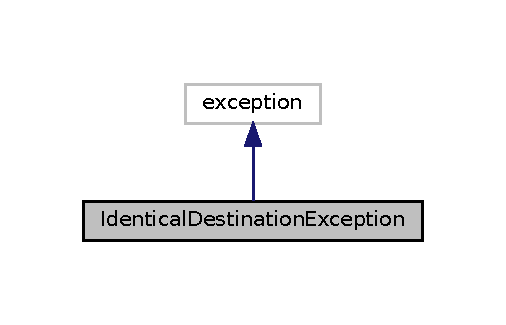
\includegraphics[width=243pt]{classIdenticalDestinationException__inherit__graph}
\end{center}
\end{figure}


Collaboration diagram for Identical\+Destination\+Exception\+:
\nopagebreak
\begin{figure}[H]
\begin{center}
\leavevmode
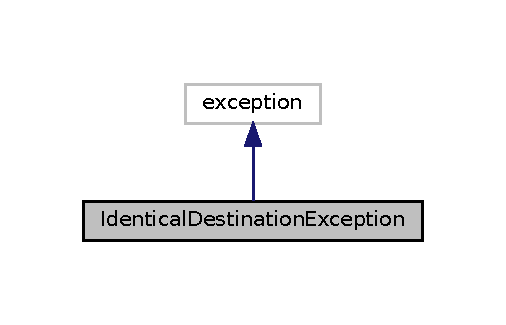
\includegraphics[width=243pt]{classIdenticalDestinationException__coll__graph}
\end{center}
\end{figure}
\subsection*{Public Member Functions}
\begin{DoxyCompactItemize}
\item 
const char $\ast$ \mbox{\hyperlink{classIdenticalDestinationException_ae07860f180405086788815185b3525b1}{what}} ()
\end{DoxyCompactItemize}


\subsection{Detailed Description}
Exception reporting when a trip has destination identical to source. 

\subsection{Member Function Documentation}
\mbox{\Hypertarget{classIdenticalDestinationException_ae07860f180405086788815185b3525b1}\label{classIdenticalDestinationException_ae07860f180405086788815185b3525b1}} 
\index{Identical\+Destination\+Exception@{Identical\+Destination\+Exception}!what@{what}}
\index{what@{what}!Identical\+Destination\+Exception@{Identical\+Destination\+Exception}}
\subsubsection{\texorpdfstring{what()}{what()}}
{\footnotesize\ttfamily const char $\ast$ Identical\+Destination\+Exception\+::what (\begin{DoxyParamCaption}{ }\end{DoxyParamCaption})}



The documentation for this class was generated from the following files\+:\begin{DoxyCompactItemize}
\item 
exceptions/\mbox{\hyperlink{IdenticalDestinationException_8h}{Identical\+Destination\+Exception.\+h}}\item 
exceptions/\mbox{\hyperlink{IdenticalDestinationException_8cpp}{Identical\+Destination\+Exception.\+cpp}}\end{DoxyCompactItemize}

\hypertarget{classInvalidDateException}{}\section{Invalid\+Date\+Exception Class Reference}
\label{classInvalidDateException}\index{Invalid\+Date\+Exception@{Invalid\+Date\+Exception}}
Inheritance diagram for Invalid\+Date\+Exception\+:\begin{figure}[H]
\begin{center}
\leavevmode
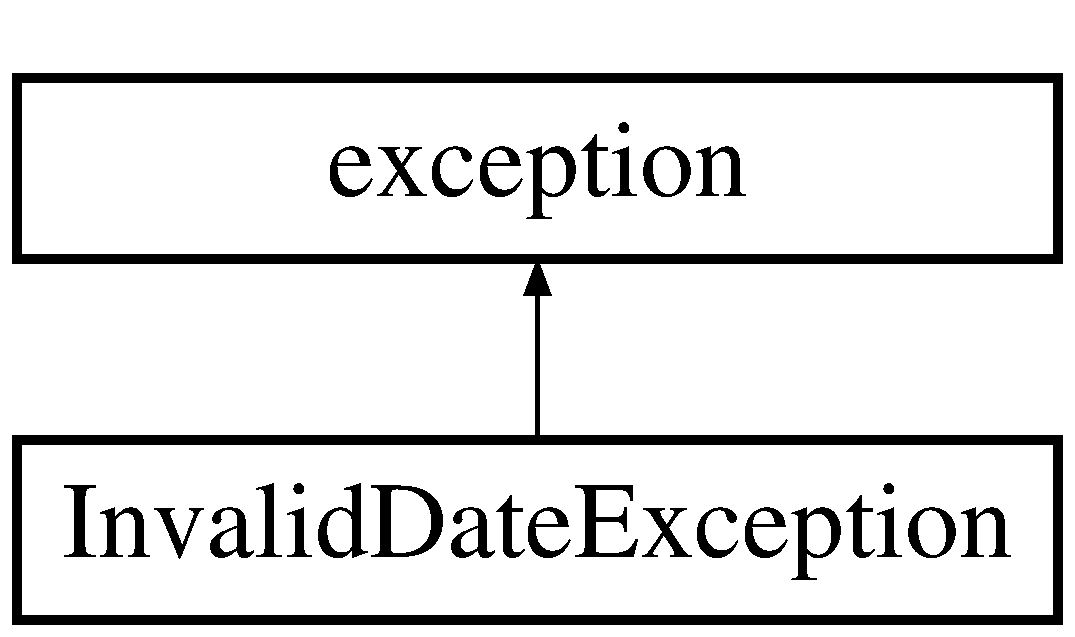
\includegraphics[height=3.000000cm]{classInvalidDateException}
\end{center}
\end{figure}
\subsection*{Public Member Functions}
\begin{DoxyCompactItemize}
\item 
\mbox{\Hypertarget{classInvalidDateException_a0ae7a8a97c0442fc025cb63e3b86bee8}\label{classInvalidDateException_a0ae7a8a97c0442fc025cb63e3b86bee8}} 
{\bfseries Invalid\+Date\+Exception} (std\+::string date\+String)
\item 
\mbox{\Hypertarget{classInvalidDateException_a518618417b66ea59ef6d5a40aad7d045}\label{classInvalidDateException_a518618417b66ea59ef6d5a40aad7d045}} 
std\+::string {\bfseries what} ()
\end{DoxyCompactItemize}
\subsection*{Public Attributes}
\begin{DoxyCompactItemize}
\item 
\mbox{\Hypertarget{classInvalidDateException_a70664a8f1fe8853eed11199c5c0f0060}\label{classInvalidDateException_a70664a8f1fe8853eed11199c5c0f0060}} 
std\+::string {\bfseries date\+String}
\end{DoxyCompactItemize}


The documentation for this class was generated from the following files\+:\begin{DoxyCompactItemize}
\item 
Invalid\+Date\+Exception.\+h\item 
Invalid\+Date\+Exception.\+cpp\end{DoxyCompactItemize}

\hypertarget{classNoSuchPassengerException}{}\section{No\+Such\+Passenger\+Exception Class Reference}
\label{classNoSuchPassengerException}\index{No\+Such\+Passenger\+Exception@{No\+Such\+Passenger\+Exception}}


Exception reporting that a passenger ID does not exist in the system.  




{\ttfamily \#include $<$No\+Such\+Passenger\+Exception.\+h$>$}

Inheritance diagram for No\+Such\+Passenger\+Exception\+:\begin{figure}[H]
\begin{center}
\leavevmode
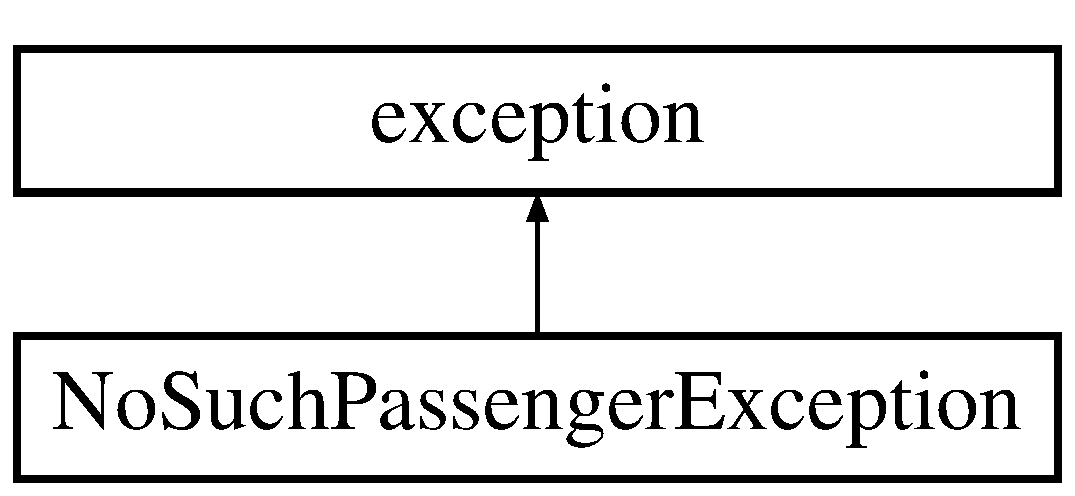
\includegraphics[height=3.000000cm]{classNoSuchPassengerException}
\end{center}
\end{figure}
\subsection*{Public Member Functions}
\begin{DoxyCompactItemize}
\item 
\mbox{\Hypertarget{classNoSuchPassengerException_a592e57495c93657a25e7da49da5b6649}\label{classNoSuchPassengerException_a592e57495c93657a25e7da49da5b6649}} 
{\bfseries No\+Such\+Passenger\+Exception} (id\+\_\+t id)
\item 
\mbox{\Hypertarget{classNoSuchPassengerException_a27bf9b4347fee63ddc405d58d217d82e}\label{classNoSuchPassengerException_a27bf9b4347fee63ddc405d58d217d82e}} 
std\+::string {\bfseries what} ()
\end{DoxyCompactItemize}


\subsection{Detailed Description}
Exception reporting that a passenger ID does not exist in the system. 

The documentation for this class was generated from the following files\+:\begin{DoxyCompactItemize}
\item 
No\+Such\+Passenger\+Exception.\+h\item 
No\+Such\+Passenger\+Exception.\+cpp\end{DoxyCompactItemize}

\hypertarget{classNoSuchStationException}{}\section{No\+Such\+Station\+Exception Class Reference}
\label{classNoSuchStationException}\index{No\+Such\+Station\+Exception@{No\+Such\+Station\+Exception}}
Inheritance diagram for No\+Such\+Station\+Exception\+:\begin{figure}[H]
\begin{center}
\leavevmode
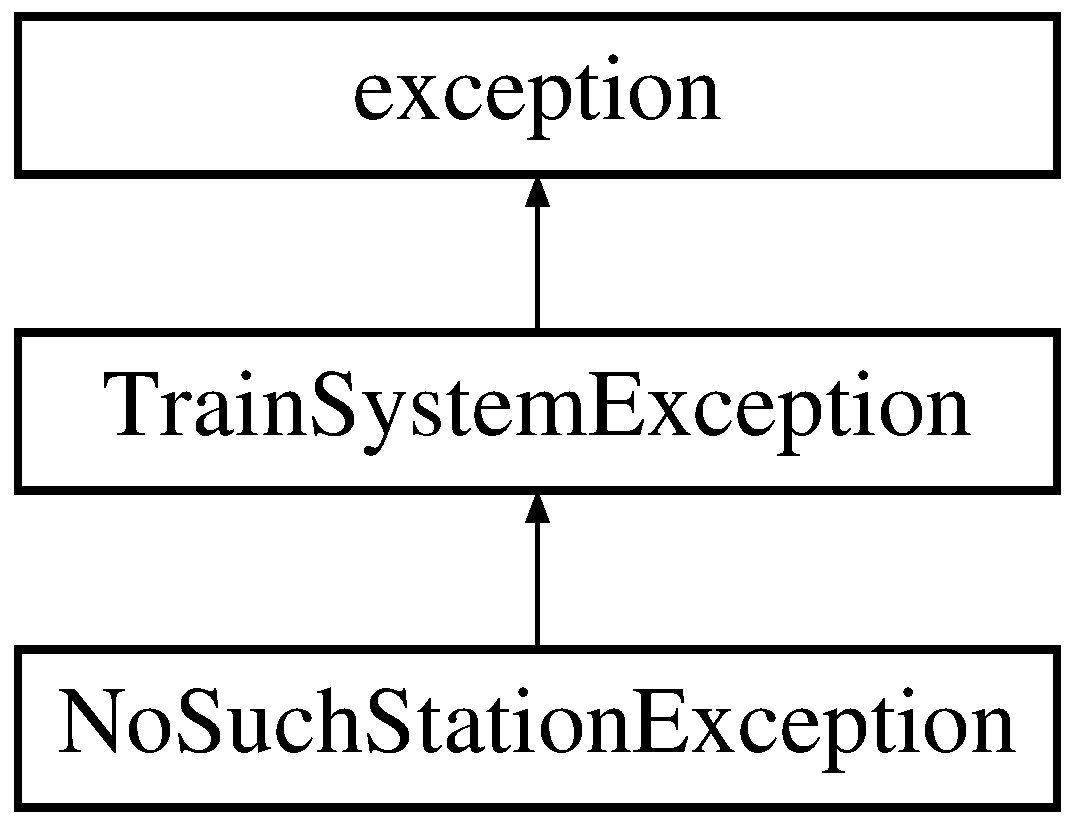
\includegraphics[height=3.000000cm]{classNoSuchStationException}
\end{center}
\end{figure}
\subsection*{Public Member Functions}
\begin{DoxyCompactItemize}
\item 
\mbox{\Hypertarget{classNoSuchStationException_a3e907e61f0836f6954f40bd63538bcb6}\label{classNoSuchStationException_a3e907e61f0836f6954f40bd63538bcb6}} 
{\bfseries No\+Such\+Station\+Exception} (id\+\_\+t id)
\item 
\mbox{\Hypertarget{classNoSuchStationException_aef7808e1393d0ed22d130fa05d20d8f7}\label{classNoSuchStationException_aef7808e1393d0ed22d130fa05d20d8f7}} 
std\+::string {\bfseries what} ()
\end{DoxyCompactItemize}


The documentation for this class was generated from the following files\+:\begin{DoxyCompactItemize}
\item 
No\+Such\+Station\+Exception.\+h\item 
No\+Such\+Station\+Exception.\+cpp\end{DoxyCompactItemize}

\hypertarget{classNoSuchTrainException}{}\section{No\+Such\+Train\+Exception Class Reference}
\label{classNoSuchTrainException}\index{No\+Such\+Train\+Exception@{No\+Such\+Train\+Exception}}


Exception reporting that a train ID does not exist in the system.  




{\ttfamily \#include $<$No\+Such\+Train\+Exception.\+h$>$}

Inheritance diagram for No\+Such\+Train\+Exception\+:\begin{figure}[H]
\begin{center}
\leavevmode
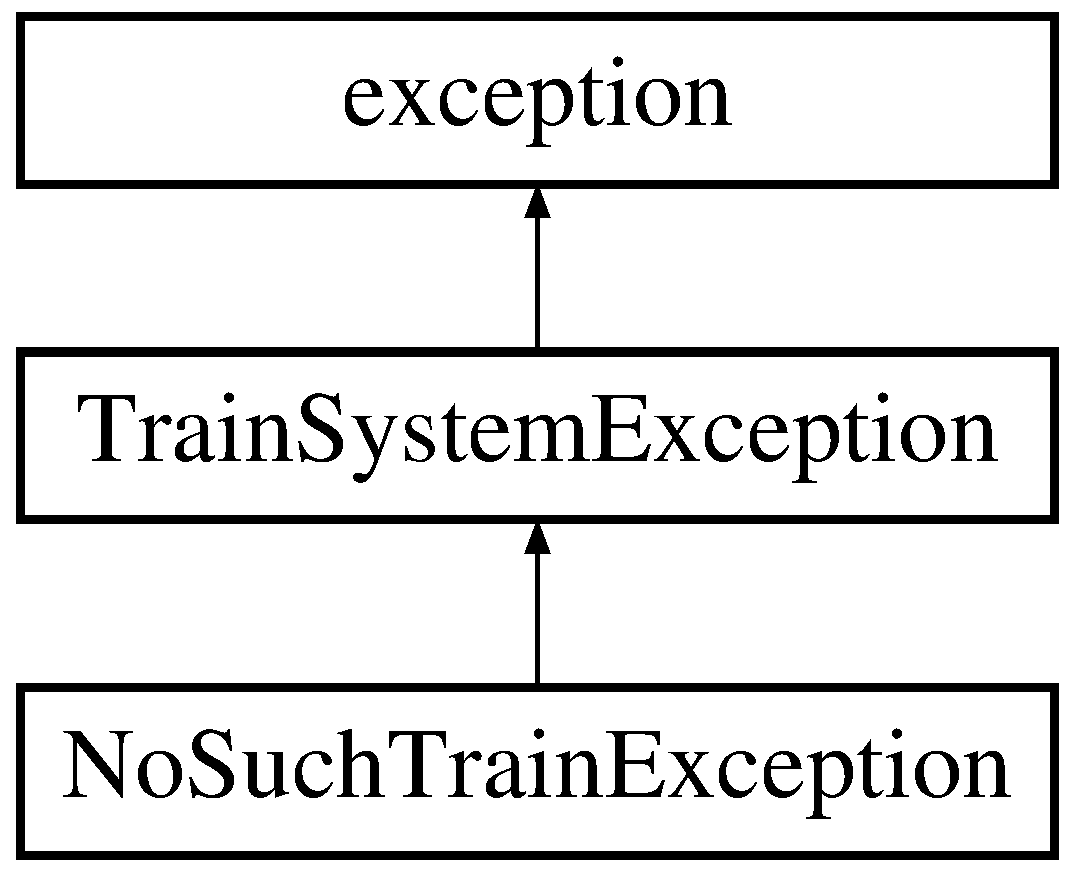
\includegraphics[height=3.000000cm]{classNoSuchTrainException}
\end{center}
\end{figure}
\subsection*{Public Member Functions}
\begin{DoxyCompactItemize}
\item 
\mbox{\Hypertarget{classNoSuchTrainException_ae60439498bd6e552159ed1c50335daba}\label{classNoSuchTrainException_ae60439498bd6e552159ed1c50335daba}} 
{\bfseries No\+Such\+Train\+Exception} (id\+\_\+t id)
\item 
\mbox{\Hypertarget{classNoSuchTrainException_a812ae27b54620f59e0a9e23969935099}\label{classNoSuchTrainException_a812ae27b54620f59e0a9e23969935099}} 
std\+::string {\bfseries what} ()
\end{DoxyCompactItemize}


\subsection{Detailed Description}
Exception reporting that a train ID does not exist in the system. 

The documentation for this class was generated from the following files\+:\begin{DoxyCompactItemize}
\item 
No\+Such\+Train\+Exception.\+h\item 
No\+Such\+Train\+Exception.\+cpp\end{DoxyCompactItemize}

\hypertarget{classNoSuchTripException}{}\section{No\+Such\+Trip\+Exception Class Reference}
\label{classNoSuchTripException}\index{No\+Such\+Trip\+Exception@{No\+Such\+Trip\+Exception}}


Exception reporting that a trip ID does not exist in the system.  




{\ttfamily \#include $<$No\+Such\+Trip\+Exception.\+h$>$}



Inheritance diagram for No\+Such\+Trip\+Exception\+:
\nopagebreak
\begin{figure}[H]
\begin{center}
\leavevmode
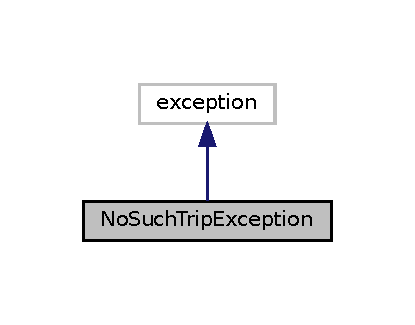
\includegraphics[width=199pt]{classNoSuchTripException__inherit__graph}
\end{center}
\end{figure}


Collaboration diagram for No\+Such\+Trip\+Exception\+:
\nopagebreak
\begin{figure}[H]
\begin{center}
\leavevmode
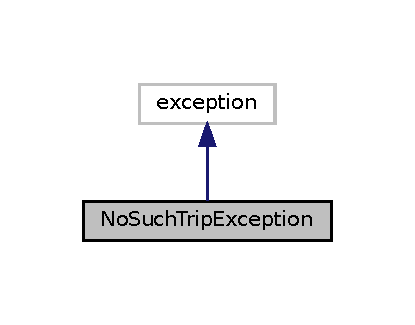
\includegraphics[width=199pt]{classNoSuchTripException__coll__graph}
\end{center}
\end{figure}
\subsection*{Public Member Functions}
\begin{DoxyCompactItemize}
\item 
\mbox{\hyperlink{classNoSuchTripException_ad4e2e75706508833ccbb7a793092734c}{No\+Such\+Trip\+Exception}} (\mbox{\hyperlink{project__utils_8h_a8f3a969054ad2200720b96e7e23dd4e1}{id\+\_\+t}} id)
\item 
const char $\ast$ \mbox{\hyperlink{classNoSuchTripException_a48adffc40883e044fd248f1185084bb6}{what}} ()
\end{DoxyCompactItemize}


\subsection{Detailed Description}
Exception reporting that a trip ID does not exist in the system. 

\subsection{Constructor \& Destructor Documentation}
\mbox{\Hypertarget{classNoSuchTripException_ad4e2e75706508833ccbb7a793092734c}\label{classNoSuchTripException_ad4e2e75706508833ccbb7a793092734c}} 
\index{No\+Such\+Trip\+Exception@{No\+Such\+Trip\+Exception}!No\+Such\+Trip\+Exception@{No\+Such\+Trip\+Exception}}
\index{No\+Such\+Trip\+Exception@{No\+Such\+Trip\+Exception}!No\+Such\+Trip\+Exception@{No\+Such\+Trip\+Exception}}
\subsubsection{\texorpdfstring{No\+Such\+Trip\+Exception()}{NoSuchTripException()}}
{\footnotesize\ttfamily No\+Such\+Trip\+Exception\+::\+No\+Such\+Trip\+Exception (\begin{DoxyParamCaption}\item[{\mbox{\hyperlink{project__utils_8h_a8f3a969054ad2200720b96e7e23dd4e1}{id\+\_\+t}}}]{id }\end{DoxyParamCaption})}



\subsection{Member Function Documentation}
\mbox{\Hypertarget{classNoSuchTripException_a48adffc40883e044fd248f1185084bb6}\label{classNoSuchTripException_a48adffc40883e044fd248f1185084bb6}} 
\index{No\+Such\+Trip\+Exception@{No\+Such\+Trip\+Exception}!what@{what}}
\index{what@{what}!No\+Such\+Trip\+Exception@{No\+Such\+Trip\+Exception}}
\subsubsection{\texorpdfstring{what()}{what()}}
{\footnotesize\ttfamily const char $\ast$ No\+Such\+Trip\+Exception\+::what (\begin{DoxyParamCaption}{ }\end{DoxyParamCaption})}



The documentation for this class was generated from the following files\+:\begin{DoxyCompactItemize}
\item 
exceptions/\mbox{\hyperlink{NoSuchTripException_8h}{No\+Such\+Trip\+Exception.\+h}}\item 
exceptions/\mbox{\hyperlink{NoSuchTripException_8cpp}{No\+Such\+Trip\+Exception.\+cpp}}\end{DoxyCompactItemize}

\hypertarget{classPassenger}{}\section{Passenger Class Reference}
\label{classPassenger}\index{Passenger@{Passenger}}
\subsection*{Public Member Functions}
\begin{DoxyCompactItemize}
\item 
\mbox{\Hypertarget{classPassenger_a895d7a9cfd358b566ed78e0d81d37bff}\label{classPassenger_a895d7a9cfd358b566ed78e0d81d37bff}} 
{\bfseries Passenger} (std\+::string name, std\+::string birth\+Date)
\item 
\mbox{\Hypertarget{classPassenger_ae6fcc19037be144f654c623c5b78ae24}\label{classPassenger_ae6fcc19037be144f654c623c5b78ae24}} 
id\+\_\+t {\bfseries get\+ID} () const
\item 
\mbox{\Hypertarget{classPassenger_a7c919f6947817ff1c6a4ee51923c116f}\label{classPassenger_a7c919f6947817ff1c6a4ee51923c116f}} 
std\+::string {\bfseries get\+Name} () const
\item 
\mbox{\Hypertarget{classPassenger_ae8d5310db80438702dec5f4d649289f1}\label{classPassenger_ae8d5310db80438702dec5f4d649289f1}} 
\mbox{\hyperlink{classPassengerCard}{Passenger\+Card}} $\ast$ {\bfseries get\+Card} () const
\item 
\mbox{\Hypertarget{classPassenger_aa2101584d2f0daf83ef58e0491754395}\label{classPassenger_aa2101584d2f0daf83ef58e0491754395}} 
const \mbox{\hyperlink{classDate}{Date}} \& {\bfseries get\+Birth\+Date} () const
\item 
\mbox{\Hypertarget{classPassenger_a06dfa54524d4ca1a85b1599b278fb871}\label{classPassenger_a06dfa54524d4ca1a85b1599b278fb871}} 
const std\+::vector$<$ \mbox{\hyperlink{classTrip}{Trip}} $\ast$ $>$ \& {\bfseries get\+Trips} () const
\item 
\mbox{\Hypertarget{classPassenger_a2fef29e013c88ba7a75d259cebfa655d}\label{classPassenger_a2fef29e013c88ba7a75d259cebfa655d}} 
bool {\bfseries add\+Trip} (\mbox{\hyperlink{classTrip}{Trip}} $\ast$trip)
\item 
\mbox{\Hypertarget{classPassenger_a72e4042544557a3dd9c02198aa2582d8}\label{classPassenger_a72e4042544557a3dd9c02198aa2582d8}} 
void {\bfseries print\+Row} (std\+::ostream \&os)
\end{DoxyCompactItemize}
\subsection*{Friends}
\begin{DoxyCompactItemize}
\item 
\mbox{\Hypertarget{classPassenger_a7b1aeaded08562578690b788f39db888}\label{classPassenger_a7b1aeaded08562578690b788f39db888}} 
std\+::ostream \& {\bfseries operator$<$$<$} (std\+::ostream \&os, \mbox{\hyperlink{classPassenger}{Passenger}} \&p)
\end{DoxyCompactItemize}


The documentation for this class was generated from the following files\+:\begin{DoxyCompactItemize}
\item 
Passenger.\+h\item 
Passenger.\+cpp\end{DoxyCompactItemize}

\hypertarget{classPassengerCard}{}\section{Passenger\+Card Class Reference}
\label{classPassengerCard}\index{Passenger\+Card@{Passenger\+Card}}


Class for representing the card of a passenger in the system.  




{\ttfamily \#include $<$Passenger\+Card.\+h$>$}

\subsection*{Public Types}
\begin{DoxyCompactItemize}
\item 
enum \mbox{\hyperlink{classPassengerCard_ac30388c823af514403463a797e2878af}{Card\+Type}} \{ \mbox{\hyperlink{classPassengerCard_ac30388c823af514403463a797e2878afab0b85af6d5ffb07453865fc04cae9453}{twenty\+Five}} =25, 
\mbox{\hyperlink{classPassengerCard_ac30388c823af514403463a797e2878afac443f0b05b5c1f059e4a99fef0cdea4c}{fifty}} =50, 
\mbox{\hyperlink{classPassengerCard_ac30388c823af514403463a797e2878afaa1ae2020789a526d593e7b80d4ee370d}{hundred}} =100
 \}
\begin{DoxyCompactList}\small\item\em Card Type enum. \end{DoxyCompactList}\end{DoxyCompactItemize}
\subsection*{Public Member Functions}
\begin{DoxyCompactItemize}
\item 
\mbox{\hyperlink{classPassengerCard_a1ebc730da7c0820350024f29c37ce9d9}{Passenger\+Card}} (\mbox{\hyperlink{classPassengerCard_ac30388c823af514403463a797e2878af}{Card\+Type}} type, \mbox{\hyperlink{project__utils_8h_a8f3a969054ad2200720b96e7e23dd4e1}{id\+\_\+t}} passenger\+ID, std\+::string p\+Name)
\begin{DoxyCompactList}\small\item\em Construct a new \mbox{\hyperlink{classPassenger}{Passenger}} Card object. \end{DoxyCompactList}\item 
int \mbox{\hyperlink{classPassengerCard_a62d2651d233d28643d5e0863500c42c4}{get\+Discount}} () const
\begin{DoxyCompactList}\small\item\em Get the discount percentage provided by the card. \end{DoxyCompactList}\item 
\mbox{\hyperlink{classPassengerCard_ac30388c823af514403463a797e2878af}{Card\+Type}} \mbox{\hyperlink{classPassengerCard_aef682e4bb625ac937c4aec7999c92626}{get\+Type}} ()
\begin{DoxyCompactList}\small\item\em Get the Type object. \end{DoxyCompactList}\item 
\mbox{\hyperlink{project__utils_8h_a91ad9478d81a7aaf2593e8d9c3d06a14}{uint}} \mbox{\hyperlink{classPassengerCard_a8428ca4fc3d4c7b4636be628c2fe5aad}{get\+Cost}} ()
\begin{DoxyCompactList}\small\item\em Get the monthly cost of the card. \end{DoxyCompactList}\item 
void \mbox{\hyperlink{classPassengerCard_ab0c4c67f185dc1abee907b6cd50413bf}{set\+Type}} (\mbox{\hyperlink{classPassengerCard_ac30388c823af514403463a797e2878af}{Card\+Type}} type)
\begin{DoxyCompactList}\small\item\em Set the typeof the card. \end{DoxyCompactList}\end{DoxyCompactItemize}
\subsection*{Static Public Attributes}
\begin{DoxyCompactItemize}
\item 
static \mbox{\hyperlink{project__utils_8h_a8f3a969054ad2200720b96e7e23dd4e1}{id\+\_\+t}} \mbox{\hyperlink{classPassengerCard_af557a01fde14b95c0e0b355e777e2aec}{current\+ID}} = 0
\begin{DoxyCompactList}\small\item\em Next ID Counter. \end{DoxyCompactList}\end{DoxyCompactItemize}


\subsection{Detailed Description}
Class for representing the card of a passenger in the system. 

\subsection{Member Enumeration Documentation}
\mbox{\Hypertarget{classPassengerCard_ac30388c823af514403463a797e2878af}\label{classPassengerCard_ac30388c823af514403463a797e2878af}} 
\index{Passenger\+Card@{Passenger\+Card}!Card\+Type@{Card\+Type}}
\index{Card\+Type@{Card\+Type}!Passenger\+Card@{Passenger\+Card}}
\subsubsection{\texorpdfstring{Card\+Type}{CardType}}
{\footnotesize\ttfamily enum \mbox{\hyperlink{classPassengerCard_ac30388c823af514403463a797e2878af}{Passenger\+Card\+::\+Card\+Type}}}



Card Type enum. 

\begin{DoxyEnumFields}{Enumerator}
\raisebox{\heightof{T}}[0pt][0pt]{\index{twenty\+Five@{twenty\+Five}!Passenger\+Card@{Passenger\+Card}}\index{Passenger\+Card@{Passenger\+Card}!twenty\+Five@{twenty\+Five}}}\mbox{\Hypertarget{classPassengerCard_ac30388c823af514403463a797e2878afab0b85af6d5ffb07453865fc04cae9453}\label{classPassengerCard_ac30388c823af514403463a797e2878afab0b85af6d5ffb07453865fc04cae9453}} 
twenty\+Five&\\
\hline

\raisebox{\heightof{T}}[0pt][0pt]{\index{fifty@{fifty}!Passenger\+Card@{Passenger\+Card}}\index{Passenger\+Card@{Passenger\+Card}!fifty@{fifty}}}\mbox{\Hypertarget{classPassengerCard_ac30388c823af514403463a797e2878afac443f0b05b5c1f059e4a99fef0cdea4c}\label{classPassengerCard_ac30388c823af514403463a797e2878afac443f0b05b5c1f059e4a99fef0cdea4c}} 
fifty&\\
\hline

\raisebox{\heightof{T}}[0pt][0pt]{\index{hundred@{hundred}!Passenger\+Card@{Passenger\+Card}}\index{Passenger\+Card@{Passenger\+Card}!hundred@{hundred}}}\mbox{\Hypertarget{classPassengerCard_ac30388c823af514403463a797e2878afaa1ae2020789a526d593e7b80d4ee370d}\label{classPassengerCard_ac30388c823af514403463a797e2878afaa1ae2020789a526d593e7b80d4ee370d}} 
hundred&\\
\hline

\end{DoxyEnumFields}


\subsection{Constructor \& Destructor Documentation}
\mbox{\Hypertarget{classPassengerCard_a1ebc730da7c0820350024f29c37ce9d9}\label{classPassengerCard_a1ebc730da7c0820350024f29c37ce9d9}} 
\index{Passenger\+Card@{Passenger\+Card}!Passenger\+Card@{Passenger\+Card}}
\index{Passenger\+Card@{Passenger\+Card}!Passenger\+Card@{Passenger\+Card}}
\subsubsection{\texorpdfstring{Passenger\+Card()}{PassengerCard()}}
{\footnotesize\ttfamily Passenger\+Card\+::\+Passenger\+Card (\begin{DoxyParamCaption}\item[{\mbox{\hyperlink{classPassengerCard_ac30388c823af514403463a797e2878af}{Card\+Type}}}]{type,  }\item[{\mbox{\hyperlink{project__utils_8h_a8f3a969054ad2200720b96e7e23dd4e1}{id\+\_\+t}}}]{passenger\+ID,  }\item[{std\+::string}]{p\+Name }\end{DoxyParamCaption})}



Construct a new \mbox{\hyperlink{classPassenger}{Passenger}} Card object. 


\begin{DoxyParams}{Parameters}
{\em type} & Type of the card \\
\hline
{\em passenger\+ID} & ID of the passenger \\
\hline
{\em p\+Name} & Name of the passenger that owns the card \\
\hline
\end{DoxyParams}


\subsection{Member Function Documentation}
\mbox{\Hypertarget{classPassengerCard_a8428ca4fc3d4c7b4636be628c2fe5aad}\label{classPassengerCard_a8428ca4fc3d4c7b4636be628c2fe5aad}} 
\index{Passenger\+Card@{Passenger\+Card}!get\+Cost@{get\+Cost}}
\index{get\+Cost@{get\+Cost}!Passenger\+Card@{Passenger\+Card}}
\subsubsection{\texorpdfstring{get\+Cost()}{getCost()}}
{\footnotesize\ttfamily \mbox{\hyperlink{project__utils_8h_a91ad9478d81a7aaf2593e8d9c3d06a14}{uint}} Passenger\+Card\+::get\+Cost (\begin{DoxyParamCaption}{ }\end{DoxyParamCaption})}



Get the monthly cost of the card. 

\begin{DoxyReturn}{Returns}
uint Monthly cost of the card in cents 
\end{DoxyReturn}
\mbox{\Hypertarget{classPassengerCard_a62d2651d233d28643d5e0863500c42c4}\label{classPassengerCard_a62d2651d233d28643d5e0863500c42c4}} 
\index{Passenger\+Card@{Passenger\+Card}!get\+Discount@{get\+Discount}}
\index{get\+Discount@{get\+Discount}!Passenger\+Card@{Passenger\+Card}}
\subsubsection{\texorpdfstring{get\+Discount()}{getDiscount()}}
{\footnotesize\ttfamily int Passenger\+Card\+::get\+Discount (\begin{DoxyParamCaption}{ }\end{DoxyParamCaption}) const}



Get the discount percentage provided by the card. 

\begin{DoxyReturn}{Returns}
int Percentag of discount 
\end{DoxyReturn}
\mbox{\Hypertarget{classPassengerCard_aef682e4bb625ac937c4aec7999c92626}\label{classPassengerCard_aef682e4bb625ac937c4aec7999c92626}} 
\index{Passenger\+Card@{Passenger\+Card}!get\+Type@{get\+Type}}
\index{get\+Type@{get\+Type}!Passenger\+Card@{Passenger\+Card}}
\subsubsection{\texorpdfstring{get\+Type()}{getType()}}
{\footnotesize\ttfamily \mbox{\hyperlink{classPassengerCard_ac30388c823af514403463a797e2878af}{Passenger\+Card\+::\+Card\+Type}} Passenger\+Card\+::get\+Type (\begin{DoxyParamCaption}{ }\end{DoxyParamCaption})}



Get the Type object. 

\begin{DoxyReturn}{Returns}
Card\+Type 
\end{DoxyReturn}
\mbox{\Hypertarget{classPassengerCard_ab0c4c67f185dc1abee907b6cd50413bf}\label{classPassengerCard_ab0c4c67f185dc1abee907b6cd50413bf}} 
\index{Passenger\+Card@{Passenger\+Card}!set\+Type@{set\+Type}}
\index{set\+Type@{set\+Type}!Passenger\+Card@{Passenger\+Card}}
\subsubsection{\texorpdfstring{set\+Type()}{setType()}}
{\footnotesize\ttfamily void Passenger\+Card\+::set\+Type (\begin{DoxyParamCaption}\item[{\mbox{\hyperlink{classPassengerCard_ac30388c823af514403463a797e2878af}{Card\+Type}}}]{type }\end{DoxyParamCaption})}



Set the typeof the card. 


\begin{DoxyParams}{Parameters}
{\em type} & \\
\hline
\end{DoxyParams}


\subsection{Member Data Documentation}
\mbox{\Hypertarget{classPassengerCard_af557a01fde14b95c0e0b355e777e2aec}\label{classPassengerCard_af557a01fde14b95c0e0b355e777e2aec}} 
\index{Passenger\+Card@{Passenger\+Card}!current\+ID@{current\+ID}}
\index{current\+ID@{current\+ID}!Passenger\+Card@{Passenger\+Card}}
\subsubsection{\texorpdfstring{current\+ID}{currentID}}
{\footnotesize\ttfamily \mbox{\hyperlink{project__utils_8h_a8f3a969054ad2200720b96e7e23dd4e1}{id\+\_\+t}} Passenger\+Card\+::current\+ID = 0\hspace{0.3cm}{\ttfamily [static]}}



Next ID Counter. 

Used to set new ID when \mbox{\hyperlink{classPassengerCard}{Passenger\+Card}} object is constructed, incremented every time a new \mbox{\hyperlink{classPassengerCard}{Passenger\+Card}} object is constructed. 

The documentation for this class was generated from the following files\+:\begin{DoxyCompactItemize}
\item 
system\+\_\+elements/\mbox{\hyperlink{PassengerCard_8h}{Passenger\+Card.\+h}}\item 
system\+\_\+elements/\mbox{\hyperlink{PassengerCard_8cpp}{Passenger\+Card.\+cpp}}\end{DoxyCompactItemize}

\hypertarget{classReverseDatesException}{}\section{Reverse\+Dates\+Exception Class Reference}
\label{classReverseDatesException}\index{Reverse\+Dates\+Exception@{Reverse\+Dates\+Exception}}


Exception reporting a trip\textquotesingle{}s arrival date happens before departure date.  




{\ttfamily \#include $<$Reverse\+Dates\+Exception.\+h$>$}



Inheritance diagram for Reverse\+Dates\+Exception\+:
\nopagebreak
\begin{figure}[H]
\begin{center}
\leavevmode
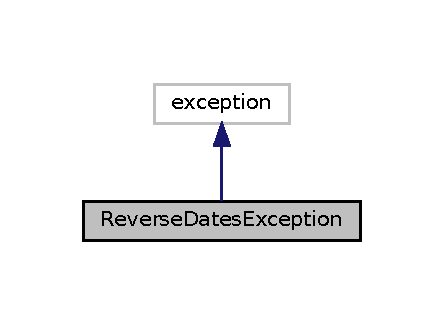
\includegraphics[width=213pt]{classReverseDatesException__inherit__graph}
\end{center}
\end{figure}


Collaboration diagram for Reverse\+Dates\+Exception\+:
\nopagebreak
\begin{figure}[H]
\begin{center}
\leavevmode
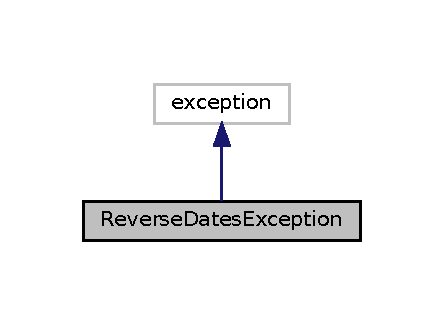
\includegraphics[width=213pt]{classReverseDatesException__coll__graph}
\end{center}
\end{figure}
\subsection*{Public Member Functions}
\begin{DoxyCompactItemize}
\item 
\mbox{\hyperlink{classReverseDatesException_afc245532384383f8f62b20358326c773}{Reverse\+Dates\+Exception}} (const std\+::string date1, const std\+::string date2)
\item 
const char $\ast$ \mbox{\hyperlink{classReverseDatesException_a52bb69fd0d940befffd9d69855ed6ae8}{what}} ()
\end{DoxyCompactItemize}


\subsection{Detailed Description}
Exception reporting a trip\textquotesingle{}s arrival date happens before departure date. 

\subsection{Constructor \& Destructor Documentation}
\mbox{\Hypertarget{classReverseDatesException_afc245532384383f8f62b20358326c773}\label{classReverseDatesException_afc245532384383f8f62b20358326c773}} 
\index{Reverse\+Dates\+Exception@{Reverse\+Dates\+Exception}!Reverse\+Dates\+Exception@{Reverse\+Dates\+Exception}}
\index{Reverse\+Dates\+Exception@{Reverse\+Dates\+Exception}!Reverse\+Dates\+Exception@{Reverse\+Dates\+Exception}}
\subsubsection{\texorpdfstring{Reverse\+Dates\+Exception()}{ReverseDatesException()}}
{\footnotesize\ttfamily Reverse\+Dates\+Exception\+::\+Reverse\+Dates\+Exception (\begin{DoxyParamCaption}\item[{const std\+::string}]{date1,  }\item[{const std\+::string}]{date2 }\end{DoxyParamCaption})}



\subsection{Member Function Documentation}
\mbox{\Hypertarget{classReverseDatesException_a52bb69fd0d940befffd9d69855ed6ae8}\label{classReverseDatesException_a52bb69fd0d940befffd9d69855ed6ae8}} 
\index{Reverse\+Dates\+Exception@{Reverse\+Dates\+Exception}!what@{what}}
\index{what@{what}!Reverse\+Dates\+Exception@{Reverse\+Dates\+Exception}}
\subsubsection{\texorpdfstring{what()}{what()}}
{\footnotesize\ttfamily const char $\ast$ Reverse\+Dates\+Exception\+::what (\begin{DoxyParamCaption}{ }\end{DoxyParamCaption})}



The documentation for this class was generated from the following files\+:\begin{DoxyCompactItemize}
\item 
exceptions/\mbox{\hyperlink{ReverseDatesException_8h}{Reverse\+Dates\+Exception.\+h}}\item 
exceptions/\mbox{\hyperlink{ReverseDatesException_8cpp}{Reverse\+Dates\+Exception.\+cpp}}\end{DoxyCompactItemize}

\hypertarget{classStation}{}\section{Station Class Reference}
\label{classStation}\index{Station@{Station}}


Class for representing a station in the system.  




{\ttfamily \#include $<$Station.\+h$>$}

\subsection*{Public Member Functions}
\begin{DoxyCompactItemize}
\item 
\mbox{\hyperlink{classStation_a53a471eb11c9431c3e89058d558f7601}{Station}} (std\+::string name)
\begin{DoxyCompactList}\small\item\em Construct a new \mbox{\hyperlink{classStation}{Station}} object. \end{DoxyCompactList}\item 
id\+\_\+t \mbox{\hyperlink{classStation_acbc5832d77cbe29c9006212b9cc32a42}{get\+ID}} () const
\begin{DoxyCompactList}\small\item\em Get the station ID. \end{DoxyCompactList}\item 
std\+::string \mbox{\hyperlink{classStation_ac823ae175ec0e2baff462ed9612c7bae}{get\+Name}} () const
\begin{DoxyCompactList}\small\item\em Get the \mbox{\hyperlink{classStation}{Station}}\textquotesingle{}s name. \end{DoxyCompactList}\item 
void \mbox{\hyperlink{classStation_a66c028cdffd79bddd0704235b051ff4e}{print\+Row}} (std\+::ostream \&os)
\begin{DoxyCompactList}\small\item\em Output station information in a row fashion. \end{DoxyCompactList}\end{DoxyCompactItemize}
\subsection*{Friends}
\begin{DoxyCompactItemize}
\item 
std\+::ostream \& \mbox{\hyperlink{classStation_ae5ca3266f8eead5634eb5926438392da}{operator$<$$<$}} (std\+::ostream \&os, \mbox{\hyperlink{classStation}{Station}} \&st)
\begin{DoxyCompactList}\small\item\em Output \mbox{\hyperlink{classStation}{Station}} object in a user friendly fashion. \end{DoxyCompactList}\end{DoxyCompactItemize}


\subsection{Detailed Description}
Class for representing a station in the system. 

\subsection{Constructor \& Destructor Documentation}
\mbox{\Hypertarget{classStation_a53a471eb11c9431c3e89058d558f7601}\label{classStation_a53a471eb11c9431c3e89058d558f7601}} 
\index{Station@{Station}!Station@{Station}}
\index{Station@{Station}!Station@{Station}}
\subsubsection{\texorpdfstring{Station()}{Station()}}
{\footnotesize\ttfamily Station\+::\+Station (\begin{DoxyParamCaption}\item[{std\+::string}]{name }\end{DoxyParamCaption})}



Construct a new \mbox{\hyperlink{classStation}{Station}} object. 


\begin{DoxyParams}{Parameters}
{\em name} & Name of the station. \\
\hline
\end{DoxyParams}


\subsection{Member Function Documentation}
\mbox{\Hypertarget{classStation_acbc5832d77cbe29c9006212b9cc32a42}\label{classStation_acbc5832d77cbe29c9006212b9cc32a42}} 
\index{Station@{Station}!get\+ID@{get\+ID}}
\index{get\+ID@{get\+ID}!Station@{Station}}
\subsubsection{\texorpdfstring{get\+I\+D()}{getID()}}
{\footnotesize\ttfamily id\+\_\+t Station\+::get\+ID (\begin{DoxyParamCaption}{ }\end{DoxyParamCaption}) const}



Get the station ID. 

\begin{DoxyReturn}{Returns}
id\+\_\+t 
\end{DoxyReturn}
\mbox{\Hypertarget{classStation_ac823ae175ec0e2baff462ed9612c7bae}\label{classStation_ac823ae175ec0e2baff462ed9612c7bae}} 
\index{Station@{Station}!get\+Name@{get\+Name}}
\index{get\+Name@{get\+Name}!Station@{Station}}
\subsubsection{\texorpdfstring{get\+Name()}{getName()}}
{\footnotesize\ttfamily string Station\+::get\+Name (\begin{DoxyParamCaption}{ }\end{DoxyParamCaption}) const}



Get the \mbox{\hyperlink{classStation}{Station}}\textquotesingle{}s name. 

\begin{DoxyReturn}{Returns}
std\+::string \mbox{\hyperlink{classStation}{Station}}\textquotesingle{}s name 
\end{DoxyReturn}
\mbox{\Hypertarget{classStation_a66c028cdffd79bddd0704235b051ff4e}\label{classStation_a66c028cdffd79bddd0704235b051ff4e}} 
\index{Station@{Station}!print\+Row@{print\+Row}}
\index{print\+Row@{print\+Row}!Station@{Station}}
\subsubsection{\texorpdfstring{print\+Row()}{printRow()}}
{\footnotesize\ttfamily void Station\+::print\+Row (\begin{DoxyParamCaption}\item[{std\+::ostream \&}]{os }\end{DoxyParamCaption})}



Output station information in a row fashion. 

Outputs the object\textquotesingle{}s information as it was a row in a table. Useful for outputing all \mbox{\hyperlink{classStation}{Station}} objects in the system.


\begin{DoxyParams}{Parameters}
{\em os} & The output stream to which the station will be output. \\
\hline
\end{DoxyParams}


\subsection{Friends And Related Function Documentation}
\mbox{\Hypertarget{classStation_ae5ca3266f8eead5634eb5926438392da}\label{classStation_ae5ca3266f8eead5634eb5926438392da}} 
\index{Station@{Station}!operator$<$$<$@{operator$<$$<$}}
\index{operator$<$$<$@{operator$<$$<$}!Station@{Station}}
\subsubsection{\texorpdfstring{operator$<$$<$}{operator<<}}
{\footnotesize\ttfamily std\+::ostream\& operator$<$$<$ (\begin{DoxyParamCaption}\item[{std\+::ostream \&}]{os,  }\item[{\mbox{\hyperlink{classStation}{Station}} \&}]{st }\end{DoxyParamCaption})\hspace{0.3cm}{\ttfamily [friend]}}



Output \mbox{\hyperlink{classStation}{Station}} object in a user friendly fashion. 


\begin{DoxyParams}{Parameters}
{\em os} & Output stream to wich \mbox{\hyperlink{classStation}{Station}} object will be output \\
\hline
{\em p} & \mbox{\hyperlink{classStation}{Station}} object to be output \\
\hline
\end{DoxyParams}
\begin{DoxyReturn}{Returns}
std\+::ostream\& 
\end{DoxyReturn}


The documentation for this class was generated from the following files\+:\begin{DoxyCompactItemize}
\item 
Station.\+h\item 
Station.\+cpp\end{DoxyCompactItemize}

\hypertarget{classSystem}{}\section{System Class Reference}
\label{classSystem}\index{System@{System}}
\subsection*{Public Member Functions}
\begin{DoxyCompactItemize}
\item 
\mbox{\Hypertarget{classSystem_aa4879a70a434d3b879090500b282de0b}\label{classSystem_aa4879a70a434d3b879090500b282de0b}} 
std\+::vector$<$ \mbox{\hyperlink{classPassenger}{Passenger}} $\ast$ $>$ \& {\bfseries get\+Passengers} ()
\item 
\mbox{\Hypertarget{classSystem_a97b3ac8c8d84fecbdd2c49df5e4b51bf}\label{classSystem_a97b3ac8c8d84fecbdd2c49df5e4b51bf}} 
std\+::vector$<$ \mbox{\hyperlink{classTrip}{Trip}} $\ast$ $>$ \& {\bfseries get\+Trips} ()
\item 
\mbox{\Hypertarget{classSystem_a44ee205bcb6c27bb1a7bc7fb545aef44}\label{classSystem_a44ee205bcb6c27bb1a7bc7fb545aef44}} 
std\+::vector$<$ \mbox{\hyperlink{classTrain}{Train}} $\ast$ $>$ \& {\bfseries get\+Trains} ()
\item 
\mbox{\Hypertarget{classSystem_a6f27512fba42cc093efd34fe10bf0045}\label{classSystem_a6f27512fba42cc093efd34fe10bf0045}} 
std\+::vector$<$ \mbox{\hyperlink{classStation}{Station}} $\ast$ $>$ \& {\bfseries get\+Stations} ()
\item 
\mbox{\Hypertarget{classSystem_a5a0348802d5cdb666f330b1e10d32727}\label{classSystem_a5a0348802d5cdb666f330b1e10d32727}} 
\mbox{\hyperlink{classPassenger}{Passenger}} $\ast$ {\bfseries get\+Passenger} (const id\+\_\+t id)
\item 
\mbox{\Hypertarget{classSystem_a518ff04299c8b37d3cbec814ac0b7ec6}\label{classSystem_a518ff04299c8b37d3cbec814ac0b7ec6}} 
\mbox{\hyperlink{classTrip}{Trip}} $\ast$ {\bfseries get\+Trip} (const id\+\_\+t id)
\item 
\mbox{\Hypertarget{classSystem_ac29b91a9dca7dd1bb4c39769a75d444f}\label{classSystem_ac29b91a9dca7dd1bb4c39769a75d444f}} 
\mbox{\hyperlink{classTrain}{Train}} $\ast$ {\bfseries get\+Train} (const id\+\_\+t id)
\item 
\mbox{\Hypertarget{classSystem_aaadc55451a0d43b7ba98ff5377de8e02}\label{classSystem_aaadc55451a0d43b7ba98ff5377de8e02}} 
\mbox{\hyperlink{classStation}{Station}} $\ast$ {\bfseries get\+Station} (const id\+\_\+t id)
\item 
\mbox{\Hypertarget{classSystem_a231710db7f31b3fec68f90fd90b292eb}\label{classSystem_a231710db7f31b3fec68f90fd90b292eb}} 
int {\bfseries get\+Station\+Index} (id\+\_\+t station\+ID)
\item 
\mbox{\Hypertarget{classSystem_a15d033a2efda45b83bbe0800698ae712}\label{classSystem_a15d033a2efda45b83bbe0800698ae712}} 
int {\bfseries get\+Train\+Index} (id\+\_\+t train\+ID)
\item 
\mbox{\Hypertarget{classSystem_aa431fdc152458fc39efb9a60e9f62f01}\label{classSystem_aa431fdc152458fc39efb9a60e9f62f01}} 
int {\bfseries get\+Trip\+Index} (id\+\_\+t trip\+ID)
\item 
\mbox{\Hypertarget{classSystem_a293b247432ab577c9bf0ba7285a6eeda}\label{classSystem_a293b247432ab577c9bf0ba7285a6eeda}} 
std\+::vector$<$ \mbox{\hyperlink{classTrip}{Trip}} $\ast$ $>$ {\bfseries search\+Trips} (\mbox{\hyperlink{classStation}{Station}} $\ast$src, \mbox{\hyperlink{classStation}{Station}} $\ast$dest, bool search\+By\+Arrival\+Date, \mbox{\hyperlink{classDate}{Date}} arrival\+Date)
\item 
\mbox{\Hypertarget{classSystem_a933891c246bf870518f334ea5666b95c}\label{classSystem_a933891c246bf870518f334ea5666b95c}} 
bool {\bfseries add\+Passenger} (\mbox{\hyperlink{classPassenger}{Passenger}} $\ast$passenger)
\item 
\mbox{\Hypertarget{classSystem_ad019d3f8d30be9b2f57842512f0393ed}\label{classSystem_ad019d3f8d30be9b2f57842512f0393ed}} 
bool {\bfseries add\+Trip} (\mbox{\hyperlink{classTrip}{Trip}} $\ast$trip)
\item 
\mbox{\Hypertarget{classSystem_a8022adc1c1f212c138ca9da7995bb422}\label{classSystem_a8022adc1c1f212c138ca9da7995bb422}} 
bool {\bfseries add\+Train} (\mbox{\hyperlink{classTrain}{Train}} $\ast$train)
\item 
\mbox{\Hypertarget{classSystem_abc5bda005d56392c66914ddd4f96e725}\label{classSystem_abc5bda005d56392c66914ddd4f96e725}} 
bool {\bfseries add\+Station} (\mbox{\hyperlink{classStation}{Station}} $\ast$station)
\item 
\mbox{\Hypertarget{classSystem_af31acdda711986978533367ce3a64276}\label{classSystem_af31acdda711986978533367ce3a64276}} 
bool {\bfseries remove\+Passenger} (id\+\_\+t id)
\item 
\mbox{\Hypertarget{classSystem_ae802cde42ae56b50adc02c76920e9001}\label{classSystem_ae802cde42ae56b50adc02c76920e9001}} 
bool {\bfseries remove\+Trip} (id\+\_\+t id)
\item 
\mbox{\Hypertarget{classSystem_ae582dd1c79cbd879ba1fbec5ceaab2fb}\label{classSystem_ae582dd1c79cbd879ba1fbec5ceaab2fb}} 
bool {\bfseries remove\+Station} (id\+\_\+t id)
\item 
\mbox{\Hypertarget{classSystem_acf1d845cdb88b43143b3f738214e866b}\label{classSystem_acf1d845cdb88b43143b3f738214e866b}} 
bool {\bfseries remove\+Train} (id\+\_\+t id)
\item 
\mbox{\Hypertarget{classSystem_a623d7369872a9af9b69b24bd2a3c71b1}\label{classSystem_a623d7369872a9af9b69b24bd2a3c71b1}} 
void {\bfseries create\+Passenger} (std\+::string name, \mbox{\hyperlink{classDate}{Date}} birth\+Date)
\item 
\mbox{\Hypertarget{classSystem_a9e317da5b607c6dee850089f340dd9e7}\label{classSystem_a9e317da5b607c6dee850089f340dd9e7}} 
void {\bfseries create\+Card} (\mbox{\hyperlink{classPassenger}{Passenger}} $\ast$p, std\+::string type)
\item 
\mbox{\Hypertarget{classSystem_ab8cf1529f497af79b72fe6cc59b08d60}\label{classSystem_ab8cf1529f497af79b72fe6cc59b08d60}} 
void {\bfseries create\+Station} (std\+::string name)
\item 
\mbox{\Hypertarget{classSystem_aa4cf09119e31e5bdf9d9187a7a60cd1a}\label{classSystem_aa4cf09119e31e5bdf9d9187a7a60cd1a}} 
void {\bfseries create\+Train} (uint max\+Seats)
\item 
\mbox{\Hypertarget{classSystem_aea8519bf009400085f8e499891b7eb37}\label{classSystem_aea8519bf009400085f8e499891b7eb37}} 
void {\bfseries create\+Trip} (uint base\+Price, \mbox{\hyperlink{classStation}{Station}} $\ast$source, \mbox{\hyperlink{classStation}{Station}} $\ast$destination, \mbox{\hyperlink{classTrain}{Train}} $\ast$train, const \mbox{\hyperlink{classDate}{Date}} daparture\+Date, const \mbox{\hyperlink{classDate}{Date}} arrival\+Date)
\item 
\mbox{\Hypertarget{classSystem_a360f9d625dbc649d567249642c1db53c}\label{classSystem_a360f9d625dbc649d567249642c1db53c}} 
void {\bfseries sort\+Passengers} ()
\item 
\mbox{\Hypertarget{classSystem_ae3b7301dda5863379777c863df0b976e}\label{classSystem_ae3b7301dda5863379777c863df0b976e}} 
void {\bfseries sort\+Passengers\+By\+Name} ()
\item 
\mbox{\Hypertarget{classSystem_a94f061c2fa79b7f0e4f175fc68a59246}\label{classSystem_a94f061c2fa79b7f0e4f175fc68a59246}} 
void {\bfseries sort\+Stations} ()
\item 
\mbox{\Hypertarget{classSystem_a3961bbb1e8a309ef37c4366731bbb813}\label{classSystem_a3961bbb1e8a309ef37c4366731bbb813}} 
void {\bfseries sort\+Trains} ()
\item 
\mbox{\Hypertarget{classSystem_a9122a0e24a88b5111959fdc87b23bc6b}\label{classSystem_a9122a0e24a88b5111959fdc87b23bc6b}} 
void {\bfseries sort\+Trips} ()
\item 
\mbox{\Hypertarget{classSystem_a3a2aace3c50cfbf7f9d2354cd858a59b}\label{classSystem_a3a2aace3c50cfbf7f9d2354cd858a59b}} 
void {\bfseries sort\+Trips\+By\+Date} ()
\item 
\mbox{\Hypertarget{classSystem_ac2b6f3d934b64f4fa56ffb1db1d261df}\label{classSystem_ac2b6f3d934b64f4fa56ffb1db1d261df}} 
bool {\bfseries process\+Ticket\+Purchase\+Request} (\mbox{\hyperlink{classTicketPurchaseRequest}{Ticket\+Purchase\+Request}} \&request)
\item 
\mbox{\Hypertarget{classSystem_aebffe11376f68cb17175f30ea517c10b}\label{classSystem_aebffe11376f68cb17175f30ea517c10b}} 
void {\bfseries process\+Cards} ()
\item 
\mbox{\Hypertarget{classSystem_ae5df9c6b2309272f8642cb16dbe5132e}\label{classSystem_ae5df9c6b2309272f8642cb16dbe5132e}} 
bool {\bfseries pay\+Card} (id\+\_\+t passenger\+ID)
\item 
\mbox{\Hypertarget{classSystem_a23c0b01d0e84fa4665ce85203ce6747b}\label{classSystem_a23c0b01d0e84fa4665ce85203ce6747b}} 
void {\bfseries list\+Passengers} (std\+::ostream \&os)
\item 
\mbox{\Hypertarget{classSystem_a06041827a7b47ad06eee9d121e42590c}\label{classSystem_a06041827a7b47ad06eee9d121e42590c}} 
void {\bfseries list\+Stations} (std\+::ostream \&os)
\item 
\mbox{\Hypertarget{classSystem_a0a6c0d8d1061893151f9b4ee3332ce85}\label{classSystem_a0a6c0d8d1061893151f9b4ee3332ce85}} 
void {\bfseries list\+Trains} (std\+::ostream \&os)
\item 
\mbox{\Hypertarget{classSystem_af11f201f6417c2658f35238d98c6f032}\label{classSystem_af11f201f6417c2658f35238d98c6f032}} 
void {\bfseries list\+Trips} (std\+::ostream \&os)
\item 
\mbox{\Hypertarget{classSystem_a1c5753d5c70d15dc3fe56fd5e421ba76}\label{classSystem_a1c5753d5c70d15dc3fe56fd5e421ba76}} 
void {\bfseries print\+Passengers} (std\+::ostream \&os) const
\item 
\mbox{\Hypertarget{classSystem_ac4b65c4fe2628e7d35b1027161e9d1da}\label{classSystem_ac4b65c4fe2628e7d35b1027161e9d1da}} 
void {\bfseries print\+Stations} (std\+::ostream \&os) const
\item 
\mbox{\Hypertarget{classSystem_af4610f38d80e01a18f2083a7c5fbd5ce}\label{classSystem_af4610f38d80e01a18f2083a7c5fbd5ce}} 
void {\bfseries print\+Trains} (std\+::ostream \&os) const
\item 
\mbox{\Hypertarget{classSystem_abaa61b6377abcfc61da32092e5d734d9}\label{classSystem_abaa61b6377abcfc61da32092e5d734d9}} 
void {\bfseries print\+Trips} (std\+::ostream \&os) const
\item 
\mbox{\Hypertarget{classSystem_aaad47fd0e1bf746a0bed32feb9553e53}\label{classSystem_aaad47fd0e1bf746a0bed32feb9553e53}} 
void {\bfseries print\+Sales} (std\+::ostream \&os) const
\end{DoxyCompactItemize}
\subsection*{Static Public Attributes}
\begin{DoxyCompactItemize}
\item 
\mbox{\Hypertarget{classSystem_a40d348884d1b737ecd26b4bc6509bf48}\label{classSystem_a40d348884d1b737ecd26b4bc6509bf48}} 
static \mbox{\hyperlink{classSystem}{System}} {\bfseries instance} = \mbox{\hyperlink{classSystem}{System}}()
\end{DoxyCompactItemize}
\subsection*{Friends}
\begin{DoxyCompactItemize}
\item 
\mbox{\Hypertarget{classSystem_a1efa95132e95a7a6b11c3b54916d66ae}\label{classSystem_a1efa95132e95a7a6b11c3b54916d66ae}} 
std\+::ostream \& {\bfseries operator$<$$<$} (std\+::ostream \&os, \mbox{\hyperlink{classSystem}{System}} \&sys)
\end{DoxyCompactItemize}


The documentation for this class was generated from the following files\+:\begin{DoxyCompactItemize}
\item 
System.\+h\item 
System.\+cpp\end{DoxyCompactItemize}

\hypertarget{classTicketInvoice}{}\section{Ticket\+Invoice Class Reference}
\label{classTicketInvoice}\index{Ticket\+Invoice@{Ticket\+Invoice}}


Class for representing an invoice of a ticket purchase in the system.  




{\ttfamily \#include $<$Ticket\+Invoice.\+h$>$}

\subsection*{Public Member Functions}
\begin{DoxyCompactItemize}
\item 
\mbox{\hyperlink{classTicketInvoice_a38b37e5168ce71bbf37aceef8a6f6267}{Ticket\+Invoice}} (\mbox{\hyperlink{classPassenger}{Passenger}} $\ast$p, \mbox{\hyperlink{classTrip}{Trip}} $\ast$t)
\begin{DoxyCompactList}\small\item\em Construct a new Ticket Invoice object. \end{DoxyCompactList}\item 
const std\+::string \mbox{\hyperlink{classTicketInvoice_a9fdfdcd08ff90480ca85e027f57033e4}{get\+Passenger\+Name}} () const
\begin{DoxyCompactList}\small\item\em Get the \mbox{\hyperlink{classPassenger}{Passenger}} Name. \end{DoxyCompactList}\item 
const std\+::string \mbox{\hyperlink{classTicketInvoice_ad692197170d5cb11790dff71150ef891}{get\+Source\+Name}} () const
\begin{DoxyCompactList}\small\item\em Get the Source Name. \end{DoxyCompactList}\item 
const std\+::string \mbox{\hyperlink{classTicketInvoice_a1db4ffac81e11b765c6204278a3df8ff}{get\+Dest\+Name}} () const
\begin{DoxyCompactList}\small\item\em Get the Dest Name. \end{DoxyCompactList}\item 
const std\+::string \mbox{\hyperlink{classTicketInvoice_a97998091765f01ff9f394210530a89ed}{get\+Price\+String}} () const
\begin{DoxyCompactList}\small\item\em Get the Price String. \end{DoxyCompactList}\item 
const \mbox{\hyperlink{project__utils_8h_a91ad9478d81a7aaf2593e8d9c3d06a14}{uint}} \mbox{\hyperlink{classTicketInvoice_a3758bface685702a6229d617691663e1}{get\+Price}} () const
\begin{DoxyCompactList}\small\item\em Get the Price. \end{DoxyCompactList}\item 
void \mbox{\hyperlink{classTicketInvoice_afeed9962f0276861876a001e372d2063}{set\+Price}} (\mbox{\hyperlink{project__utils_8h_a91ad9478d81a7aaf2593e8d9c3d06a14}{uint}} price)
\begin{DoxyCompactList}\small\item\em Set the Price. \end{DoxyCompactList}\end{DoxyCompactItemize}
\subsection*{Friends}
\begin{DoxyCompactItemize}
\item 
std\+::ostream \& \mbox{\hyperlink{classTicketInvoice_ae78ba81ba79ed7e8c9e8cd23a910f00d}{operator$<$$<$}} (std\+::ostream \&os, \mbox{\hyperlink{classTicketInvoice}{Ticket\+Invoice}} \&in)
\end{DoxyCompactItemize}


\subsection{Detailed Description}
Class for representing an invoice of a ticket purchase in the system. 

\subsection{Constructor \& Destructor Documentation}
\mbox{\Hypertarget{classTicketInvoice_a38b37e5168ce71bbf37aceef8a6f6267}\label{classTicketInvoice_a38b37e5168ce71bbf37aceef8a6f6267}} 
\index{Ticket\+Invoice@{Ticket\+Invoice}!Ticket\+Invoice@{Ticket\+Invoice}}
\index{Ticket\+Invoice@{Ticket\+Invoice}!Ticket\+Invoice@{Ticket\+Invoice}}
\subsubsection{\texorpdfstring{Ticket\+Invoice()}{TicketInvoice()}}
{\footnotesize\ttfamily Ticket\+Invoice\+::\+Ticket\+Invoice (\begin{DoxyParamCaption}\item[{\mbox{\hyperlink{classPassenger}{Passenger}} $\ast$}]{p,  }\item[{\mbox{\hyperlink{classTrip}{Trip}} $\ast$}]{t }\end{DoxyParamCaption})}



Construct a new Ticket Invoice object. 


\begin{DoxyParams}{Parameters}
{\em p} & Pointer to the passanger that has done the purchase \\
\hline
{\em t} & \mbox{\hyperlink{classTrip}{Trip}} to which the ticket has been purchased \\
\hline
\end{DoxyParams}
Here is the call graph for this function\+:
\nopagebreak
\begin{figure}[H]
\begin{center}
\leavevmode
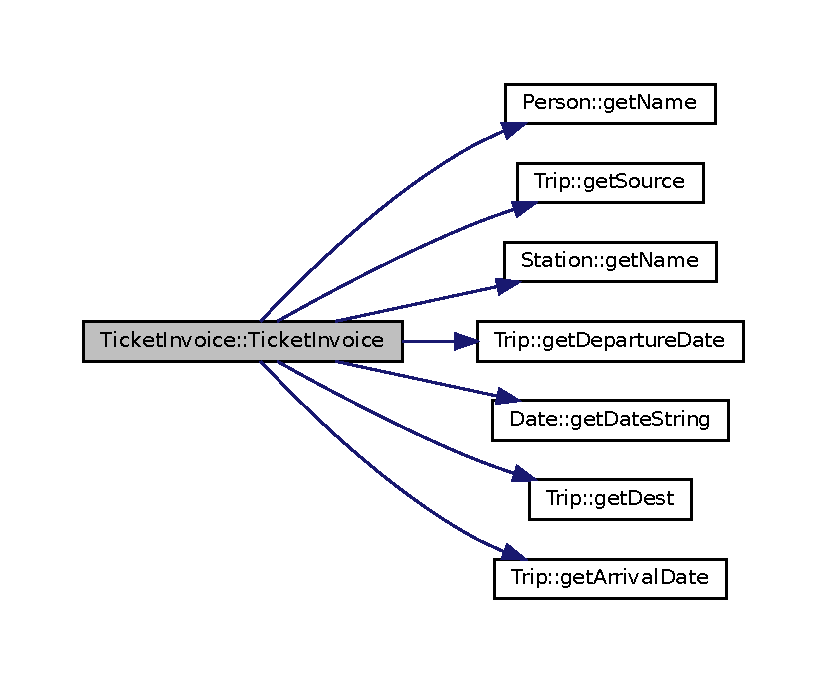
\includegraphics[width=350pt]{classTicketInvoice_a38b37e5168ce71bbf37aceef8a6f6267_cgraph}
\end{center}
\end{figure}


\subsection{Member Function Documentation}
\mbox{\Hypertarget{classTicketInvoice_a1db4ffac81e11b765c6204278a3df8ff}\label{classTicketInvoice_a1db4ffac81e11b765c6204278a3df8ff}} 
\index{Ticket\+Invoice@{Ticket\+Invoice}!get\+Dest\+Name@{get\+Dest\+Name}}
\index{get\+Dest\+Name@{get\+Dest\+Name}!Ticket\+Invoice@{Ticket\+Invoice}}
\subsubsection{\texorpdfstring{get\+Dest\+Name()}{getDestName()}}
{\footnotesize\ttfamily const string Ticket\+Invoice\+::get\+Dest\+Name (\begin{DoxyParamCaption}{ }\end{DoxyParamCaption}) const}



Get the Dest Name. 

\begin{DoxyReturn}{Returns}
const std\+::string Name of the destination station 
\end{DoxyReturn}
\mbox{\Hypertarget{classTicketInvoice_a9fdfdcd08ff90480ca85e027f57033e4}\label{classTicketInvoice_a9fdfdcd08ff90480ca85e027f57033e4}} 
\index{Ticket\+Invoice@{Ticket\+Invoice}!get\+Passenger\+Name@{get\+Passenger\+Name}}
\index{get\+Passenger\+Name@{get\+Passenger\+Name}!Ticket\+Invoice@{Ticket\+Invoice}}
\subsubsection{\texorpdfstring{get\+Passenger\+Name()}{getPassengerName()}}
{\footnotesize\ttfamily const string Ticket\+Invoice\+::get\+Passenger\+Name (\begin{DoxyParamCaption}{ }\end{DoxyParamCaption}) const}



Get the \mbox{\hyperlink{classPassenger}{Passenger}} Name. 

\begin{DoxyReturn}{Returns}
const std\+::string Name of the passenger 
\end{DoxyReturn}
\mbox{\Hypertarget{classTicketInvoice_a3758bface685702a6229d617691663e1}\label{classTicketInvoice_a3758bface685702a6229d617691663e1}} 
\index{Ticket\+Invoice@{Ticket\+Invoice}!get\+Price@{get\+Price}}
\index{get\+Price@{get\+Price}!Ticket\+Invoice@{Ticket\+Invoice}}
\subsubsection{\texorpdfstring{get\+Price()}{getPrice()}}
{\footnotesize\ttfamily const \mbox{\hyperlink{project__utils_8h_a91ad9478d81a7aaf2593e8d9c3d06a14}{uint}} Ticket\+Invoice\+::get\+Price (\begin{DoxyParamCaption}{ }\end{DoxyParamCaption}) const}



Get the Price. 

\begin{DoxyReturn}{Returns}
const uint The price in cents 
\end{DoxyReturn}
\mbox{\Hypertarget{classTicketInvoice_a97998091765f01ff9f394210530a89ed}\label{classTicketInvoice_a97998091765f01ff9f394210530a89ed}} 
\index{Ticket\+Invoice@{Ticket\+Invoice}!get\+Price\+String@{get\+Price\+String}}
\index{get\+Price\+String@{get\+Price\+String}!Ticket\+Invoice@{Ticket\+Invoice}}
\subsubsection{\texorpdfstring{get\+Price\+String()}{getPriceString()}}
{\footnotesize\ttfamily const string Ticket\+Invoice\+::get\+Price\+String (\begin{DoxyParamCaption}{ }\end{DoxyParamCaption}) const}



Get the Price String. 

\begin{DoxyReturn}{Returns}
const std\+::string A string representing the price in euros(not cents) 
\end{DoxyReturn}
\mbox{\Hypertarget{classTicketInvoice_ad692197170d5cb11790dff71150ef891}\label{classTicketInvoice_ad692197170d5cb11790dff71150ef891}} 
\index{Ticket\+Invoice@{Ticket\+Invoice}!get\+Source\+Name@{get\+Source\+Name}}
\index{get\+Source\+Name@{get\+Source\+Name}!Ticket\+Invoice@{Ticket\+Invoice}}
\subsubsection{\texorpdfstring{get\+Source\+Name()}{getSourceName()}}
{\footnotesize\ttfamily const string Ticket\+Invoice\+::get\+Source\+Name (\begin{DoxyParamCaption}{ }\end{DoxyParamCaption}) const}



Get the Source Name. 

\begin{DoxyReturn}{Returns}
const std\+::string Name of the source station 
\end{DoxyReturn}
\mbox{\Hypertarget{classTicketInvoice_afeed9962f0276861876a001e372d2063}\label{classTicketInvoice_afeed9962f0276861876a001e372d2063}} 
\index{Ticket\+Invoice@{Ticket\+Invoice}!set\+Price@{set\+Price}}
\index{set\+Price@{set\+Price}!Ticket\+Invoice@{Ticket\+Invoice}}
\subsubsection{\texorpdfstring{set\+Price()}{setPrice()}}
{\footnotesize\ttfamily void Ticket\+Invoice\+::set\+Price (\begin{DoxyParamCaption}\item[{\mbox{\hyperlink{project__utils_8h_a91ad9478d81a7aaf2593e8d9c3d06a14}{uint}}}]{price }\end{DoxyParamCaption})}



Set the Price. 


\begin{DoxyParams}{Parameters}
{\em price} & \\
\hline
\end{DoxyParams}


\subsection{Friends And Related Function Documentation}
\mbox{\Hypertarget{classTicketInvoice_ae78ba81ba79ed7e8c9e8cd23a910f00d}\label{classTicketInvoice_ae78ba81ba79ed7e8c9e8cd23a910f00d}} 
\index{Ticket\+Invoice@{Ticket\+Invoice}!operator$<$$<$@{operator$<$$<$}}
\index{operator$<$$<$@{operator$<$$<$}!Ticket\+Invoice@{Ticket\+Invoice}}
\subsubsection{\texorpdfstring{operator$<$$<$}{operator<<}}
{\footnotesize\ttfamily std\+::ostream\& operator$<$$<$ (\begin{DoxyParamCaption}\item[{std\+::ostream \&}]{os,  }\item[{\mbox{\hyperlink{classTicketInvoice}{Ticket\+Invoice}} \&}]{in }\end{DoxyParamCaption})\hspace{0.3cm}{\ttfamily [friend]}}



The documentation for this class was generated from the following files\+:\begin{DoxyCompactItemize}
\item 
\mbox{\hyperlink{TicketInvoice_8h}{Ticket\+Invoice.\+h}}\item 
\mbox{\hyperlink{TicketInvoice_8cpp}{Ticket\+Invoice.\+cpp}}\end{DoxyCompactItemize}

\hypertarget{classTicketPurchaseRequest}{}\section{Ticket\+Purchase\+Request Class Reference}
\label{classTicketPurchaseRequest}\index{Ticket\+Purchase\+Request@{Ticket\+Purchase\+Request}}
\subsection*{Public Member Functions}
\begin{DoxyCompactItemize}
\item 
\mbox{\Hypertarget{classTicketPurchaseRequest_aaa01be19b8a8ef88428f4d1dc3a3c63c}\label{classTicketPurchaseRequest_aaa01be19b8a8ef88428f4d1dc3a3c63c}} 
{\bfseries Ticket\+Purchase\+Request} (\mbox{\hyperlink{classPassenger}{Passenger}} $\ast$passenger, \mbox{\hyperlink{classTrip}{Trip}} $\ast$t)
\item 
\mbox{\Hypertarget{classTicketPurchaseRequest_a08428a7617aa26c16702420e61ce0312}\label{classTicketPurchaseRequest_a08428a7617aa26c16702420e61ce0312}} 
const \mbox{\hyperlink{classPassenger}{Passenger}} $\ast$ {\bfseries get\+Passenger} () const
\item 
\mbox{\Hypertarget{classTicketPurchaseRequest_a7ae48dcccbcddb298fae1bd74048570b}\label{classTicketPurchaseRequest_a7ae48dcccbcddb298fae1bd74048570b}} 
const \mbox{\hyperlink{classTrip}{Trip}} $\ast$ {\bfseries get\+Trip} () const
\item 
\mbox{\Hypertarget{classTicketPurchaseRequest_a289ba4fd54f5a0e5a8e8e4eecbff6b23}\label{classTicketPurchaseRequest_a289ba4fd54f5a0e5a8e8e4eecbff6b23}} 
void {\bfseries set\+Price} (uint price)
\item 
\mbox{\Hypertarget{classTicketPurchaseRequest_a626107dad44c79663d318573e5c6bae2}\label{classTicketPurchaseRequest_a626107dad44c79663d318573e5c6bae2}} 
void {\bfseries print\+Invoice} (std\+::ostream \&os)
\end{DoxyCompactItemize}
\subsection*{Friends}
\begin{DoxyCompactItemize}
\item 
\mbox{\Hypertarget{classTicketPurchaseRequest_af18a9ee98e70982bfe2975391d7221a5}\label{classTicketPurchaseRequest_af18a9ee98e70982bfe2975391d7221a5}} 
class {\bfseries System}
\end{DoxyCompactItemize}


The documentation for this class was generated from the following files\+:\begin{DoxyCompactItemize}
\item 
Ticket\+Purchase\+Request.\+h\item 
Ticket\+Purchase\+Request.\+cpp\end{DoxyCompactItemize}

\hypertarget{classTrain}{}\section{Train Class Reference}
\label{classTrain}\index{Train@{Train}}


Class for representing a train in the system.  




{\ttfamily \#include $<$Train.\+h$>$}

\subsection*{Public Member Functions}
\begin{DoxyCompactItemize}
\item 
\mbox{\hyperlink{classTrain_aa965be5e5d076d2743301c5d75ce4401}{Train}} (uint total\+Seats)
\begin{DoxyCompactList}\small\item\em Construct a new \mbox{\hyperlink{classTrain}{Train}} object. \end{DoxyCompactList}\item 
id\+\_\+t \mbox{\hyperlink{classTrain_a7310ae0bc5b43ea392e4fa62630ee56b}{get\+ID}} () const
\begin{DoxyCompactList}\small\item\em Get the train ID. \end{DoxyCompactList}\item 
uint \mbox{\hyperlink{classTrain_a93cd372664bac4ba28fa36e40316444a}{get\+Max\+Seats}} ()
\begin{DoxyCompactList}\small\item\em Get the max capacity. \end{DoxyCompactList}\item 
void \mbox{\hyperlink{classTrain_a3fd1c87c2152aa96cc6928f0aea37e21}{print\+Row}} (std\+::ostream \&os)
\begin{DoxyCompactList}\small\item\em Output train information in a row fashion. \end{DoxyCompactList}\end{DoxyCompactItemize}
\subsection*{Friends}
\begin{DoxyCompactItemize}
\item 
\mbox{\Hypertarget{classTrain_ab4c39558eb319a2f509b128f1fc90bd8}\label{classTrain_ab4c39558eb319a2f509b128f1fc90bd8}} 
std\+::ostream \& {\bfseries operator$<$$<$} (std\+::ostream \&os, \mbox{\hyperlink{classTrain}{Train}} \&tr)
\end{DoxyCompactItemize}


\subsection{Detailed Description}
Class for representing a train in the system. 

\subsection{Constructor \& Destructor Documentation}
\mbox{\Hypertarget{classTrain_aa965be5e5d076d2743301c5d75ce4401}\label{classTrain_aa965be5e5d076d2743301c5d75ce4401}} 
\index{Train@{Train}!Train@{Train}}
\index{Train@{Train}!Train@{Train}}
\subsubsection{\texorpdfstring{Train()}{Train()}}
{\footnotesize\ttfamily Train\+::\+Train (\begin{DoxyParamCaption}\item[{uint}]{total\+Seats }\end{DoxyParamCaption})}



Construct a new \mbox{\hyperlink{classTrain}{Train}} object. 


\begin{DoxyParams}{Parameters}
{\em total\+Seats} & Max capacity of train \\
\hline
\end{DoxyParams}


\subsection{Member Function Documentation}
\mbox{\Hypertarget{classTrain_a7310ae0bc5b43ea392e4fa62630ee56b}\label{classTrain_a7310ae0bc5b43ea392e4fa62630ee56b}} 
\index{Train@{Train}!get\+ID@{get\+ID}}
\index{get\+ID@{get\+ID}!Train@{Train}}
\subsubsection{\texorpdfstring{get\+I\+D()}{getID()}}
{\footnotesize\ttfamily id\+\_\+t Train\+::get\+ID (\begin{DoxyParamCaption}{ }\end{DoxyParamCaption}) const}



Get the train ID. 

\begin{DoxyReturn}{Returns}
id\+\_\+t 
\end{DoxyReturn}
\mbox{\Hypertarget{classTrain_a93cd372664bac4ba28fa36e40316444a}\label{classTrain_a93cd372664bac4ba28fa36e40316444a}} 
\index{Train@{Train}!get\+Max\+Seats@{get\+Max\+Seats}}
\index{get\+Max\+Seats@{get\+Max\+Seats}!Train@{Train}}
\subsubsection{\texorpdfstring{get\+Max\+Seats()}{getMaxSeats()}}
{\footnotesize\ttfamily uint Train\+::get\+Max\+Seats (\begin{DoxyParamCaption}{ }\end{DoxyParamCaption})}



Get the max capacity. 

\begin{DoxyReturn}{Returns}
uint 
\end{DoxyReturn}
\mbox{\Hypertarget{classTrain_a3fd1c87c2152aa96cc6928f0aea37e21}\label{classTrain_a3fd1c87c2152aa96cc6928f0aea37e21}} 
\index{Train@{Train}!print\+Row@{print\+Row}}
\index{print\+Row@{print\+Row}!Train@{Train}}
\subsubsection{\texorpdfstring{print\+Row()}{printRow()}}
{\footnotesize\ttfamily void Train\+::print\+Row (\begin{DoxyParamCaption}\item[{std\+::ostream \&}]{os }\end{DoxyParamCaption})}



Output train information in a row fashion. 

Outputs the object\textquotesingle{}s information as it was a row in a table. Useful for outputing all train objects in the system.


\begin{DoxyParams}{Parameters}
{\em os} & The output stream to which the train will be output. \\
\hline
\end{DoxyParams}


The documentation for this class was generated from the following files\+:\begin{DoxyCompactItemize}
\item 
Train.\+h\item 
Train.\+cpp\end{DoxyCompactItemize}

\hypertarget{classTrainSystemException}{}\section{Train\+System\+Exception Class Reference}
\label{classTrainSystemException}\index{Train\+System\+Exception@{Train\+System\+Exception}}
Inheritance diagram for Train\+System\+Exception\+:\begin{figure}[H]
\begin{center}
\leavevmode
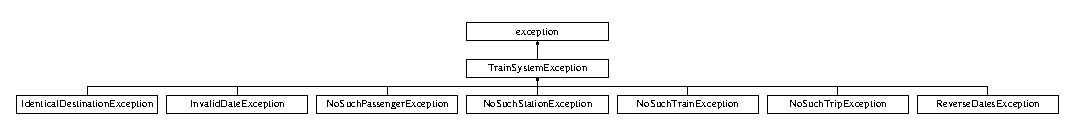
\includegraphics[height=1.304348cm]{classTrainSystemException}
\end{center}
\end{figure}
\subsection*{Public Member Functions}
\begin{DoxyCompactItemize}
\item 
\mbox{\Hypertarget{classTrainSystemException_a9f4952ed02d47ffa66abd0c9627a7975}\label{classTrainSystemException_a9f4952ed02d47ffa66abd0c9627a7975}} 
virtual std\+::string {\bfseries what} ()=0
\end{DoxyCompactItemize}


The documentation for this class was generated from the following file\+:\begin{DoxyCompactItemize}
\item 
Train\+System\+Exception.\+h\end{DoxyCompactItemize}

\hypertarget{classTrip}{}\section{Trip Class Reference}
\label{classTrip}\index{Trip@{Trip}}
\subsection*{Public Member Functions}
\begin{DoxyCompactItemize}
\item 
\mbox{\Hypertarget{classTrip_ad7244e90c71e27914dab013835883502}\label{classTrip_ad7244e90c71e27914dab013835883502}} 
{\bfseries Trip} (uint base\+Price, \mbox{\hyperlink{classStation}{Station}} $\ast$source, \mbox{\hyperlink{classStation}{Station}} $\ast$destination, \mbox{\hyperlink{classTrain}{Train}} $\ast$train, const std\+::string daparture\+Date, const std\+::string arrival\+Date)
\item 
\mbox{\Hypertarget{classTrip_a7770a61e1211789c80b003eeedcaa09c}\label{classTrip_a7770a61e1211789c80b003eeedcaa09c}} 
id\+\_\+t {\bfseries get\+ID} () const
\item 
\mbox{\Hypertarget{classTrip_aa356ea90590c617311c911c98aac4093}\label{classTrip_aa356ea90590c617311c911c98aac4093}} 
float {\bfseries get\+Base\+Price} () const
\item 
\mbox{\Hypertarget{classTrip_a65b45d4816c85d47ef743e7c1cfe807f}\label{classTrip_a65b45d4816c85d47ef743e7c1cfe807f}} 
\mbox{\hyperlink{classStation}{Station}} $\ast$ {\bfseries get\+Source} () const
\item 
\mbox{\Hypertarget{classTrip_a459ae85fc25404ba616fabfb4b4165f4}\label{classTrip_a459ae85fc25404ba616fabfb4b4165f4}} 
\mbox{\hyperlink{classStation}{Station}} $\ast$ {\bfseries get\+Dest} () const
\item 
\mbox{\Hypertarget{classTrip_a7595a39e9aa91e321d37b1696da50024}\label{classTrip_a7595a39e9aa91e321d37b1696da50024}} 
\mbox{\hyperlink{classTrain}{Train}} $\ast$ {\bfseries get\+Train} () const
\item 
\mbox{\Hypertarget{classTrip_ac506905deb66415b2fcee1c89579e628}\label{classTrip_ac506905deb66415b2fcee1c89579e628}} 
const \mbox{\hyperlink{classDate}{Date}} \& {\bfseries get\+Departure\+Date} () const
\item 
\mbox{\Hypertarget{classTrip_a6dddee29651df86b5a2c45bd2e1d2fc6}\label{classTrip_a6dddee29651df86b5a2c45bd2e1d2fc6}} 
const \mbox{\hyperlink{classDate}{Date}} \& {\bfseries get\+Arrival\+Date} () const
\item 
\mbox{\Hypertarget{classTrip_a00e2b65d40562051bfe4124f581a49e1}\label{classTrip_a00e2b65d40562051bfe4124f581a49e1}} 
bool {\bfseries book\+Seat} ()
\item 
\mbox{\Hypertarget{classTrip_a233bab5c803f51ee5e79c611a15699c0}\label{classTrip_a233bab5c803f51ee5e79c611a15699c0}} 
void {\bfseries print\+Row} (std\+::ostream \&os)
\end{DoxyCompactItemize}
\subsection*{Friends}
\begin{DoxyCompactItemize}
\item 
\mbox{\Hypertarget{classTrip_ad143ba29c1778aa25a53301503c3f2bd}\label{classTrip_ad143ba29c1778aa25a53301503c3f2bd}} 
std\+::ostream \& {\bfseries operator$<$$<$} (std\+::ostream \&os, \mbox{\hyperlink{classTrip}{Trip}} \&tr)
\end{DoxyCompactItemize}


The documentation for this class was generated from the following files\+:\begin{DoxyCompactItemize}
\item 
Trip.\+h\item 
Trip.\+cpp\end{DoxyCompactItemize}

%--- End generated contents ---

% Index
\backmatter
\newpage
\phantomsection
\clearemptydoublepage
\addcontentsline{toc}{chapter}{Index}
\printindex

\end{document}
